% =============================================================================
% Lecture 10b: Model Compression, Part 2 (How Few Bits?)
% Introduction to Machine Learning Systems (Volume I)
% =============================================================================
% Quantization stores each value as a small integer and a shared scale. The
% range that scale covers decides how much accuracy survives; whether fewer
% bits make the device faster depends on the resource that binds and on a
% kernel that keeps the bits packed. MobileNetV2 carries the accuracy story
% (Krishnamoorthi 2018), GPT-2 XL decoding on the phone the speed story, and
% ResNet-50 the closing deployment profile.
%
% Build: make -C slides build-10b_model_compression   (figures: images/make_figs.py)
% Plan:  lecture_map.yml and storyboard.md in this folder.
% Boundaries: Lecture 11 owns the roofline and datapaths; Lecture 12b owns
% confidence calibration; Lecture 13 owns runtime and precision selection.
% =============================================================================

\documentclass[aspectratio=169, 12pt]{beamer}
\usepackage{../../assets/beamerthememlsys}
\mlsyssetup{
  volume={Volume I},
  chapter={Chapter 10},
  chaptertitle={Model Compression, Part 2},
  logo={../../assets/img/logo-mlsysbook.png},
  instlogo={../../assets/img/logo-harvard.png},
  layer=models,
  dividerstack,
}
\usepackage[T1]{fontenc}
\usepackage[scaled=0.9]{helvet}
\usepackage{courier}
\renewcommand{\familydefault}{\sfdefault}
\usepackage{booktabs,amsmath}
\usetikzlibrary{arrows.meta,positioning}
\graphicspath{{images/}}
% Generated by calcs.py. Do not edit; edit calcs.py and rerun it.
\defval{r50_float}{75.2}
\defval{r50_tensor}{75.0}
\defval{r50_tensor_loss}{0.2}
\defval{mbv2_float}{71.9}
\defval{mbv2_tensor}{0.1}
\defval{chance_pct}{0.1}
\defval{imagenet_classes}{1{,}000}
\defval{nagel_float}{71.72}
\defval{nagel_tensor}{0.12}
\defval{r50_chapter_top1}{76.1}
\defval{gpt2_fp16_gb}{3}
\defval{gpt2_read_ms}{59}
\defval{phone_bw}{51.2}
\defval{blur_cpu_ms}{125}
\defval{blur_pruned_ms}{87}
\defval{blur_int8_ms}{20}
\defval{frame_ms}{33}
\defval{mnv2_read_ms}{0.27}
\defval{mnv2_read_share_pct}{1}
\defval{r50_read_ms}{2}
\defval{blur_fp32_mb}{14.0}
\defval{blur_pruned_mb}{10.4}
\defval{blur_int8_mb}{2.6}
\defval{fp32_exp_bits}{8}
\defval{fp32_frac_bits}{23}
\defval{bf16_exp_bits}{8}
\defval{fp16_max}{65{,}504}
\defval{e4m3_exp_bits}{4}
\defval{e4m3_frac_bits}{3}
\defval{e4m3_max}{448}
\defval{e5m2_max}{57{,}344}
\defval{int8_levels}{256}
\defval{int4_levels}{16}
\defval{int8_smaller}{4}
\defval{int4_smaller}{8}
\defval{gguf_q2_k_bits}{2}
\defval{gguf_q2_k_gb}{2.83}
\defval{gguf_q2_k_bpw}{3.35}
\defval{gguf_q3_k_m_bits}{3}
\defval{gguf_q3_k_m_gb}{3.30}
\defval{gguf_q3_k_m_bpw}{3.91}
\defval{gguf_q4_0_bits}{4}
\defval{gguf_q4_0_gb}{3.83}
\defval{gguf_q4_0_bpw}{4.54}
\defval{gguf_q4_k_m_bits}{4}
\defval{gguf_q4_k_m_gb}{4.08}
\defval{gguf_q4_k_m_bpw}{4.84}
\defval{gguf_q6_k_bits}{6}
\defval{gguf_q6_k_gb}{5.53}
\defval{gguf_q6_k_bpw}{6.56}
\defval{gguf_q8_0_bits}{8}
\defval{gguf_q8_0_gb}{7.16}
\defval{gguf_q8_0_bpw}{8.50}
\defval{llama_params_b}{6.74}
\defval{q4_block}{32}
\defval{q4_scale_bytes}{2}
\defval{q4_scale_bits}{16}
\defval{q4_code_bytes}{16}
\defval{q4_block_bytes}{18}
\defval{q4_bpw}{4.5}
\defval{q4_overhead_pct}{12.5}
\defval{q2k_block_bpw}{2.5625}
\defval{e4m3_pos}{126}
\defval{e4m3_below1}{55}
\defval{e4m3_top}{7}
\defval{e4m3_top_binade}{256}
\defval{e4m3_min}{0.002}
\defval{e4m3_min_exp}{-9}
\defval{e4m3_decades_word}{five}
\defval{int8_pos}{127}
\defval{int8_step448}{3.53}
\defval{int8_zero_below}{1.76}
\defval{e_add_fp32}{0.90}
\defval{e_add_int8}{0.03}
\defval{e_add_ratio}{30}
\defval{e_mul_ratio}{18.5}
\defval{e_mac_ratio}{15.3}
\defval{e_dram}{640}
\defval{e_dram_mac}{2{,}100}
\defval{spotter_fp32_kb}{800}
\defval{spotter_int8_kb}{200}
\defval{mcu_sram_kb}{512}
\defval{toy_alpha}{-1}
\defval{toy_neg_alpha}{1}
\defval{toy_beta}{2.5}
\defval{toy_bits}{3}
\defval{toy_bits_word}{three}
\defval{toy_outside_word}{two}
\defval{toy_levels}{8}
\defval{toy_steps}{7}
\defval{toy_range}{3.5}
\defval{toy_s}{0.5}
\defval{toy_z}{2}
\defval{toy_half}{0.25}
\defval{toy_x0}{-1.4}
\defval{toy_q0}{0}
\defval{toy_r0}{-1}
\defval{toy_x1}{-0.3}
\defval{toy_q1}{1}
\defval{toy_r1}{-0.5}
\defval{toy_x2}{0.8}
\defval{toy_q2}{4}
\defval{toy_r2}{1.0}
\defval{toy_x3}{1.6}
\defval{toy_q3}{5}
\defval{toy_r3}{1.5}
\defval{toy_x4}{2.9}
\defval{toy_q4}{7}
\defval{toy_r4}{2.5}
\defval{toy_x5}{2.2}
\defval{toy_q5}{6}
\defval{toy_r5}{2.0}
\defval{toy_err5}{0.2}
\defval{nm_alpha}{-1}
\defval{nm_neg_alpha}{1}
\defval{nm_beta}{3}
\defval{nm_bits}{8}
\defval{nm_range}{4}
\defval{nm_steps}{255}
\defval{nm_s}{0.0157}
\defval{nm_z_exact}{63.75}
\defval{nm_z}{64}
\defval{nm_nudge}{0.25}
\defval{nm_x0}{-1}
\defval{nm_q0}{0}
\defval{nm_x1}{1}
\defval{nm_q1}{128}
\defval{nm_x2}{0}
\defval{nm_q2}{64}
\defval{nm_x3}{3}
\defval{nm_q3}{255}
\defval{nm_r0}{-1.004}
\defval{nm_r0_torch}{-1.0039}
\defval{l2_max}{0.392}
\defval{l2_int_max}{127}
\defval{l2_s}{0.00309}
\defval{l2_half}{0.00154}
\defval{l2_outlier}{0.784}
\defval{l2_w0}{0.127}
\defval{l2_q0}{41}
\defval{l2_e0}{0.00045}
\defval{l2_w1}{-0.084}
\defval{l2_q1}{-27}
\defval{l2_e1}{0.00066}
\defval{l2_w2}{0.392}
\defval{l2_q2}{127}
\defval{l2_e2}{0}
\defval{l2_w3}{-0.203}
\defval{l2_q3}{-66}
\defval{l2_e3}{0.00072}
\defval{zp_sym_lo}{-1}
\defval{zp_sym_hi}{1}
\defval{zp_sym_qmin}{-127}
\defval{zp_sym_qmax}{127}
\defval{zp_asym_lo}{-0.5}
\defval{zp_asym_hi}{1.5}
\defval{zp_asym_qmin}{-128}
\defval{zp_asym_qmax}{127}
\defval{zp_asym_range}{2}
\defval{zp_asym_steps}{255}
\defval{zp_asym_z}{-64}
\defval{int8_shift}{128}
\defval{relu_hi}{6}
\defval{relu_sym_div}{127}
\defval{relu_asym_div}{255}
\defval{relu_sym_s}{0.047}
\defval{relu_asym_s}{0.024}
\defval{mbv1_float}{70.9}
\defval{mbv1_sym}{59.1}
\defval{mbv1_asym}{70.3}
\defval{mbv1_sym_cost}{11}
\defval{il_w_max}{0.75}
\defval{il_x_max}{2}
\defval{il_int_max}{127}
\defval{il_w0}{0.5}
\defval{il_x0}{1.0}
\defval{il_wq0}{85}
\defval{il_xq0}{64}
\defval{il_p0}{5{,}440}
\defval{il_w1}{-0.25}
\defval{il_x1}{2.0}
\defval{il_wq1}{-42}
\defval{il_xq1}{127}
\defval{il_p1}{-5{,}334}
\defval{il_w2}{0.75}
\defval{il_x2}{0.5}
\defval{il_wq2}{127}
\defval{il_xq2}{32}
\defval{il_p2}{4{,}064}
\defval{il_w0_ratio}{84.7}
\defval{il_x0_ratio}{63.5}
\defval{il_sum}{4{,}170}
\defval{il_readback}{0.388}
\defval{il_exact}{0.375}
\defval{il_m}{0.0118}
\defval{il_y}{49}
\defval{il_sy_div}{127}
\defval{il_headroom}{133{,}000}
\defval{il_acc_exp}{31}
\defval{clip_full}{2.5}
\defval{clip_cut}{1.1}
\defval{clip_steps}{255}
\defval{clip_full_s}{0.0098}
\defval{clip_cut_s}{0.0043}
\defval{clip_finer}{2.3}
\defval{wu_resnet50_fp32}{76.16}
\defval{wu_resnet50_max}{75.82}
\defval{wu_resnet50_entropy}{76.05}
\defval{wu_resnet50_pct_99_99}{75.98}
\defval{wu_mobilenet_fp32}{71.88}
\defval{wu_mobilenet_max}{69.41}
\defval{wu_mobilenet_entropy}{70.28}
\defval{wu_mobilenet_pct_99_99}{71.14}
\defval{wu_inception_fp32}{79.71}
\defval{wu_inception_max}{0.12}
\defval{wu_inception_entropy}{79.60}
\defval{wu_inception_pct_99_99}{79.63}
\defval{wu_efficientnet_fp32}{76.85}
\defval{wu_efficientnet_max}{22.3}
\defval{wu_efficientnet_entropy}{72.06}
\defval{wu_efficientnet_pct_99_99}{68.33}
\defval{wu_bert_fp32}{91.01}
\defval{wu_bert_max}{85.92}
\defval{wu_bert_entropy}{37.40}
\defval{wu_bert_pct_99_99}{89.59}
\defval{wu_bert_best}{90.20}
\defval{mbv2_channel}{69.8}
\defval{mbv2_qat}{71.1}
\defval{mbv2_qat_gain}{1.3}
\defval{r50_channel}{75.1}
\defval{r50_qat}{75.0}
\defval{nagel_wide}{128}
\defval{nagel_narrow}{0.5}
\defval{nagel_step}{1}
\defval{nagel_channels}{32}
\defval{awq_group}{128}
\defval{det_small_m}{125}
\defval{det_mid_b}{1.3}
\defval{det_large_b}{13}
\defval{det_fourth_b}{6.7}
\defval{det_absmax_small}{87.76}
\defval{det_absmax_large}{19.08}
\defval{det_fp32_large}{12.45}
\defval{out_b}{6.7}
\defval{out_floor_b}{6}
\defval{out_tokens_pct}{75}
\defval{out_mult}{20}
\defval{out_dims}{6}
\defval{out_threshold}{6}
\defval{cliff_8bit_gap}{2}
\defval{int4_bits}{4}
\defval{int8_bits}{8}
\defval{r50_w4_tensor}{0.2}
\defval{mbv2_w4_tensor}{0.1}
\defval{r50_w4_channel}{54.0}
\defval{mbv2_w4_channel}{0.1}
\defval{r50_w4_qat}{73.2}
\defval{mbv2_w4_qat}{62.0}
\defval{r50_w4_qat_gap}{2}
\defval{mbv2_w4_qat_gap}{10}
\defval{gptq_fp16}{8.34}
\defval{gptq_rtn4}{10.54}
\defval{gptq_4}{8.37}
\defval{gptq_rtn3_k}{7.3}
\defval{gptq_3}{8.68}
\defval{awq_fp16}{10.86}
\defval{awq_rtn}{23.54}
\defval{awq_by_weight}{22.37}
\defval{awq_by_act}{11.39}
\defval{awq_kept_pct}{1}
\defval{dec_w16_gb}{3}
\defval{dec_w4_gb}{0.75}
\defval{dec_kv_gb}{0.31}
\defval{dec_t16_gb}{3.31}
\defval{dec_t4_gb}{1.06}
\defval{dec_t16_ms}{65}
\defval{dec_t4_ms}{21}
\defval{dec_speedup}{3.1}
\defval{dec_byte_ratio}{4}
\defval{h100_int8}{1{,}979}
\defval{h100_fp16}{989}
\defval{h100_int8_x}{2}
\defval{h100_int8_x_word}{two}
\defval{gptq_fp16_ms}{230}
\defval{gptq_3bit_ms}{71}
\defval{gptq_fp16_gpus_word}{five}
\defval{gptq_3bit_gpus_word}{one}
\defval{gptq_x}{3.24}
\defval{lb_ultra_bw}{800}
\defval{lb_tg4_x}{2.30}
\defval{lb_tg8_x}{1.62}
\defval{lb_pp4_x}{0.88}
\defval{lb_file_x}{3.53}
\defval{lb_other_tg_lo}{2.63}
\defval{lb_other_tg_hi}{2.86}
\defval{lb_other_pp_lo}{0.88}
\defval{lb_other_pp_hi}{0.98}
\defval{lb_stream16}{553}
\defval{lb_stream4}{360}
\defval{dq_sep_gb}{7.06}
\defval{dq_sep_ms}{138}
\defval{dq_sep_x}{2.13}
\defval{px_fp32}{105}
\defval{px_cpu}{63}
\defval{px_dsp}{15.5}
\defval{px_cpu_x}{1.7}
\defval{px_dsp_x}{6.8}
\defval{simd_bits}{512}
\defval{simd_fp32}{16}
\defval{simd_int8}{64}
\defval{pf_fp32_top1}{76.1}
\defval{pf_int8_top1}{75.8}
\defval{pf_top1_limit}{75.5}
\defval{pf_top1_drop}{0.3}
\defval{pf_fp32_cal}{2.1}
\defval{pf_int8_cal}{3.4}
\defval{pf_cal_limit}{3.0}
\defval{pf_latency_x}{1.3}
\defval{pf_throughput_x}{5.9}
\defval{pf_energy_x}{5.9}
\defval{pf_tdp_w}{700}
\defval{p7b_b}{7}
\defval{p7b_fp16_gb}{14}
\defval{p7b_int4_gb}{3.5}
\defval{p7b_q4_gb}{3.9}
\defval{int4_bytes}{0.5}
\defval{phone_ram_gb}{8}

\setcounter{mlsystotalsections}{5}

\title{Model Compression, Part 2}
\author{Vijay Janapa Reddi}
\institute{Harvard University}
\date{}

% A large answer choice for predict and concept-question slides
\newcommand{\choice}[2]{\textbf{\textcolor{mlsysaccent}{#1}}\enspace #2}
% A highlighted answer choice, shown from overlay #1 on
\newcommand{\answer}[3]{\alt<#1->{\colorbox{mlsysaccent!15}{\choice{#2}{#3}}}{\choice{#2}{#3}}}
% A goal or takeaway line with its thumbnail
\newcommand{\thumbline}[2]{%
  \begin{minipage}[c]{2.6cm}\centering\includegraphics[width=2.5cm,height=1.05cm,keepaspectratio]{#1}\end{minipage}%
  \hspace{0.3cm}\begin{minipage}[c]{0.74\textwidth}\raggedright\normalsize #2\end{minipage}}
% A true-or-false statement card
\newcommand{\tfcard}[2]{%
  \begin{mlsyscard}{mlsysaccent}
    {\small\textbf{#1}}\\[0.05cm]
    \uncover<2->{\footnotesize\textcolor{RedLine}{\textbf{False.}} #2}%
  \end{mlsyscard}}
% Styles for the integer-layer pipeline
\tikzset{
  blk/.style={draw=#1, fill=#1!12, line width=1pt, rounded corners=2pt,
    align=center, font=\footnotesize, text=darktext, minimum height=0.85cm,
    minimum width=2.3cm},
  arr/.style={-{Stealth[length=2.2mm]}, line width=0.9pt, color=midgray},
}


\begin{document}

% =============================================================================
% TITLE AND HOOK
% =============================================================================
\mlsysnote{[0.5 min] [CORE] Read the thesis once. Say what today is: the second half of the compression chapter. Part 1 changed what the model computes (pruning, distillation, low rank). Today changes how each value is stored. It asks how few bits a value can keep, and when keeping fewer bits makes the device faster. The notes total about 71.5 minutes. Notes tagged [OPTIONAL] can be cut; cutting all of them leaves a complete lecture of about 50 minutes.}
\mlsystitle{Model Compression, Part~2}{A quantized value is a small integer and a shared scale. The range sets how much accuracy survives, and the binding resource sets whether fewer bits run faster.}{cover_model_compression_blueprint.png}

\begin{frame}{One INT8 recipe spares ResNet-50, breaks MobileNetV2}
  \mlsysactivity{Predict}{2 min}
  \begin{columns}[c]
    \begin{column}{0.50\textwidth}
      \centering\mlsyssteps[width=\textwidth,height=5.0cm,keepaspectratio]{hook_step}{3}
    \end{column}
    \begin{column}{0.48\textwidth}
      \only<1|handout:0>{\normalsize Same recipe for both: every weight and activation in 8 bits, one scale per tensor, no retraining.}%
      \uncover<2->{\small Predict MobileNetV2's top-1 after conversion:\\[0.15cm]
        \normalsize\choice{A}{about 71}\qquad\choice{B}{about 65}\\[0.1cm]
        \choice{C}{about 40}\qquad\answer{3}{D}{about 0}\\[0.25cm]}
      \uncover<3->{\small \val{chance_pct}\%: chance on \val{imagenet_classes} classes. Same 8 bits. Why?}
    \end{column}
  \end{columns}
  \mlsyscredit{Krishnamoorthi 2018, Table 3 (TensorFlow-Slim checkpoints; post-training INT8, per-layer scales); Nagel et al. 2019, Table 1, report the same collapse (\val{nagel_float} to \val{nagel_tensor}\%).}
  \note{[3 min] [CORE] Step 1: two trained ImageNet classifiers, converted with one recipe: post-training quantization, which means no retraining, every weight and activation stored as an 8-bit integer, one scale per tensor. ResNet-50 goes from \val{r50_float} to \val{r50_tensor} percent top-1. Step 2: MobileNetV2, the backbone of Part 1's blur model, starts at \val{mbv2_float} percent. ENGAGE: one minute, vote A to D. Most students pick A or B, because ResNet-50 lost only \val{r50_tensor_loss} points. Step 3: D, \val{mbv2_tensor} percent, which is chance on \val{imagenet_classes} classes. Nagel et al. 2019 measured the same collapse independently, \val{nagel_float} to \val{nagel_tensor} percent. Ask for a reason and leave it open: too few parameters to spare precision? 256 levels too few? Bad calibration images? The answer comes at minute 35, and it is none of these. WARN: this is the ImageNet classifier that serves as the backbone of the chapter's segmentation model, so say ``the blur model's backbone''. The \val{r50_float} here is this paper's ResNet-50 baseline; the chapter's table later uses \val{r50_chapter_top1} from a different checkpoint, so never compare the two.}
\end{frame}

\begin{frame}{Recall: Part 1 left one tier of the stack untouched}
  \mlsysactivity{Retrieval}{1.5 min}
  \centering
  {\Large\bfseries Close your notes.}\\[0.15cm]
  {\normalsize Which tier did Part 1 leave alone? Which budget term does each case still break?}\\[0.25cm]
  \uncover<2->{%
    \begin{minipage}[c]{0.48\textwidth}\centering
      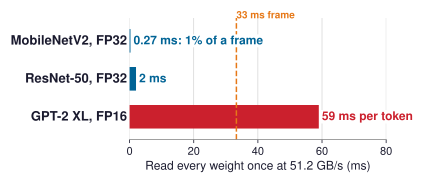
\includegraphics[width=\textwidth,height=3.6cm,keepaspectratio]{stream}\\
      {\footnotesize Decode: token time, set by weight bytes}
    \end{minipage}\hfill
    \begin{minipage}[c]{0.50\textwidth}\centering
      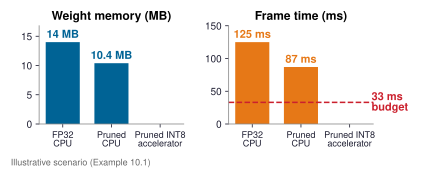
\includegraphics[width=\textwidth,height=3.6cm,keepaspectratio]{waterfall_step2}\\
      {\footnotesize Blur: frame time, still over \val{frame_ms} ms}
    \end{minipage}}
  \mlsyscredit{Model Compression, table 1 (phone bus \val{phone_bw} GB/s); Example 10.1 and the compression-waterfall figure (blur frame times, illustrative).}
  \note{[1.5 min] [CORE] ENGAGE: 45 seconds, written, notes closed. Step 2: the untouched tier is precision, how many bits each value keeps. Left: decoding GPT-2 XL on the phone reads all \val{gpt2_fp16_gb} GB of FP16 weights for every token, \val{gpt2_read_ms} ms on the \val{phone_bw} GB/s bus between memory and processor; structure did not change bytes per weight, so the token time stands. Right: channel pruning brought the blur model from \val{blur_cpu_ms} to about \val{blur_pruned_ms} ms per frame, still over the \val{frame_ms} ms budget, and the phone's integer accelerator sits unused because it cannot run FP32. Both remaining gaps are in bits per value. WARN: the blur frame times are the chapter's illustrative composite; say so. LINK: the Pixel 2 slide near minute 60 finishes the blur model's story.}
\end{frame}

\begin{frame}{How few bits can a value keep, and when does that run faster?}
  \vspace{-0.1cm}
  {\normalsize By the end of today you will be able to:}\\[0.25cm]
  \thumbline{thumb_formats_step3}{Say what each format from FP32 to INT4 spends its bits on, and what fewer bits save.}\\[0.15cm]
  \thumbline{thumb_affgrid_step3}{Quantize a tensor with a scale and a zero-point, and trace an integer layer.}\\[0.15cm]
  \thumbline{thumb_perchannel_step2}{Choose a range and a granularity, and predict when one scale per tensor fails.}\\[0.15cm]
  \thumbline{thumb_dequant_step2}{Predict when fewer bits run faster, and judge a quantized model on evidence.}\par\vspace{0.2cm}
  \threadstrip{0}{1}{0}{1}{1}
  \note{[1.5 min] [CORE] The driving question: how few bits can each value keep before accuracy breaks, and when does storing fewer bits make the device faster? Read the four outcomes; each thumbnail is the figure that teaches it. Three models run through the lecture: MobileNetV2 carries accuracy (the hook), GPT-2 XL decoding on the phone carries speed, and ResNet-50 closes with the chapter's INT8 deployment profile. The strip fills two iron-law factors: fewer bits shrink the bytes behind each FLOP (algorithm) and let integer units run faster (machine).}
\end{frame}

% =============================================================================
% SECTION: FORMATS
% =============================================================================
\mlsysnote{[0.5 min] [CORE] First the formats themselves, what a narrower number keeps and what it saves.}
\mlsysdivider{What does a narrower number keep, and what does it save?}{Model Compression, \S10.3.1, \S10.3.2}
\section{Formats}

\begin{frame}{Each format spends its bits on range, on precision, or on neither}
  \centering
  \mlsyssteps[width=0.94\textwidth,height=5.4cm,keepaspectratio]{formats_step}{3}
  \mlsyscredit{Model Compression, \S10.3.1 and table 7; FP8 limits: Micikevicius et al. 2022, Table 1. Bit fields drawn to scale.}
  \note{[2 min] [CORE] Every box is one group of bits, drawn to scale. Step 1, recall from Lecture 8b: FP32 (32-bit floating point) spends 1 sign bit, \val{fp32_exp_bits} exponent bits, and \val{fp32_frac_bits} mantissa bits. The exponent sets range (how large and how small a value can be); the mantissa sets precision (how finely values are spaced within each power of two). BF16 (brain floating point, 16 bits) keeps FP32's \val{bf16_exp_bits}-bit exponent and so its range; FP16 spends more on the mantissa and tops out at \val{fp16_max}. Step 2: two 8-bit floating-point formats. E4M3 (\val{e4m3_exp_bits} exponent, \val{e4m3_frac_bits} mantissa bits) reaches \val{e4m3_max} and is used for weights and activations; E5M2 reaches \val{e5m2_max} for the wider range of gradients. Step 3: integers have no exponent at all. INT8 is \val{int8_levels} evenly spaced levels, INT4 is \val{int4_levels}. Storage is \val{int8_smaller} and \val{int4_smaller} times smaller than FP32. ENGAGE: an integer format has no exponent; how can \val{int8_levels} levels represent a weight of 0.003 and an activation of 40? Expected: they need a scale stored alongside, the subject of the next segment. FLEX: microscaling formats (a block of 32 values shares one exponent) are reading; Lecture 13 owns runtime and precision selection.}
\end{frame}

\begin{frame}[fragile]{A real 4-bit file stores 4.5 bits or more per weight}
  \mlsysactivity{Estimate}{1 min}
  \begin{columns}[T]
    \begin{column}{0.335\textwidth}
      {\footnotesize\textbf{Llama 2 7B} files: model card}\\[0.1cm]
      \footnotesize
      \setlength{\tabcolsep}{4pt}
      \renewcommand{\arraystretch}{1.02}
      \begin{tabular}{@{}lrrr@{}}
        \toprule
        \textbf{Name} & \textbf{Bits} & \textbf{Size} & \uncover<2->{\textbf{Bits/wt}} \\[-0.05cm]
        \midrule
        Q2\_K & \val{gguf_q2_k_bits} & \val{gguf_q2_k_gb} GB & \uncover<2->{\textcolor{RedLine}{\val{gguf_q2_k_bpw}}} \\
        Q3\_K\_M & \val{gguf_q3_k_m_bits} & \val{gguf_q3_k_m_gb} GB & \uncover<2->{\val{gguf_q3_k_m_bpw}} \\
        Q4\_0 & \val{gguf_q4_0_bits} & \val{gguf_q4_0_gb} GB & \uncover<2->{\textbf{\val{gguf_q4_0_bpw}}} \\
        Q4\_K\_M & \val{gguf_q4_k_m_bits} & \val{gguf_q4_k_m_gb} GB & \uncover<2->{\val{gguf_q4_k_m_bpw}} \\
        Q6\_K & \val{gguf_q6_k_bits} & \val{gguf_q6_k_gb} GB & \uncover<2->{\val{gguf_q6_k_bpw}} \\
        Q8\_0 & \val{gguf_q8_0_bits} & \val{gguf_q8_0_gb} GB & \uncover<2->{\val{gguf_q8_0_bpw}} \\
        \bottomrule
      \end{tabular}\\[0.2cm]
      \only<1|handout:0>{\small \val{llama_params_b} billion weights in Q4\_0's \val{gguf_q4_0_gb} GB. Bits per weight?}%
      \only<2-|handout:1>{\small Every file exceeds its bits.}
    \end{column}
    \begin{column}{0.66\textwidth}
      \begin{uncoverenv}<3->
      {\footnotesize\textbf{llama.cpp}, ggml/src/ggml-common.h}
\begin{semiverbatim}\footnotesize
#define QK4_0 32
typedef struct \{
    ggml_half d;           // delta
    uint8_t qs[QK4_0 / 2]; // nibbles / quants
\} block_q4_0;
\end{semiverbatim}
      \small One \val{q4_scale_bytes}-byte scale $+$ \val{q4_code_bytes} bytes of codes\\
      $=$ \val{q4_block_bytes} bytes per \val{q4_block} weights: \textbf{\val{q4_bpw} bits per weight}
      \end{uncoverenv}
    \end{column}
  \end{columns}
  \mlsyscredit{Table: huggingface.co/TheBloke/Llama-2-7B-GGUF, Provided files (commit b4e04e1); Bits/wt: Hub byte sizes over \val{llama_params_b} B weights (calcs.py). Code: github.com/ggml-org/llama.cpp v0.7.0 (MIT).}
  \note{[2.5 min] A real artifact: the model card of a public repository of Llama 2 7B files in GGUF, the format the llama.cpp runtime loads. Step 1: three of the card's columns: the file's name, its nominal bits, and its size. ENGAGE: Q4\_0 holds \val{llama_params_b} billion weights in \val{gguf_q4_0_gb} GB; how many bits per weight? Thirty seconds. Step 2: \val{gguf_q4_0_bpw} bits (derived: bytes times 8 over the weight count). Every file is above its nominal bits. Q2\_K stores \val{gguf_q2_k_bpw} bits per weight, Q8\_0 \val{gguf_q8_0_bpw}. Step 3: why. llama.cpp's source stores weights in blocks of \val{q4_block}; each block keeps one \val{q4_scale_bits}-bit scale, d, beside \val{q4_code_bytes} bytes of packed 4-bit codes. That is \val{q4_block_bytes} bytes for \val{q4_block} weights, \val{q4_bpw} bits per weight. The scale is the price of reaching a real range with \val{int4_levels} levels, the subject of the next segment. The card's notes give Q2\_K's blocks \val{q2k_block_bpw} bits per weight; the rest of its \val{gguf_q2_k_bpw} is tensors and metadata the name does not describe. WARN: students compute INT4 bytes as parameters over two. That omits the scales, \val{q4_overhead_pct} percent more at Q4\_0; when memory is the constraint, use the file size. LINK: the closing slide's 7B model. FLEX: [OPTIONAL]; cutting it loses the real file's overhead bits.}
\end{frame}

\begin{frame}{A float grid is dense near zero; an integer grid needs a scale}
  \centering
  \mlsyssteps[width=0.94\textwidth,height=4.6cm,keepaspectratio]{grids_step}{2}\\[0.05cm]
  \uncover<2->{\small With the same 8 bits, FP8's exponent spreads its levels across \val{e4m3_decades_word} decades, and INT8 spaces its levels evenly.}
  \mlsyscredit{Derived from the FP8 E4M3 definition (Micikevicius et al. 2022, Table 1): smallest value $2^{\val{e4m3_min_exp}}$, largest \val{e4m3_max}. INT8: \val{int8_pos} positive levels.}
  \note{[1.5 min] [OPTIONAL] One log axis from 0.001 to 1,000. Step 1: every positive value FP8 E4M3 can store, one tick each: \val{e4m3_pos} values from \val{e4m3_min} to \val{e4m3_max}. Because the exponent spaces values by powers of two, \val{e4m3_below1} of them sit below 1 and only \val{e4m3_top} between \val{e4m3_top_binade} and \val{e4m3_max}. Small values get fine steps, large ones coarse steps. Step 2: INT8 asked to cover the same \val{e4m3_max}. Its \val{int8_pos} positive levels are evenly spaced, one every \val{e4m3_max} / \val{int8_pos} = \val{int8_step448}, so on a log axis they crowd at the top and nothing below \val{int8_zero_below} survives, because every such value rounds to zero. ENGAGE: which format would you rather use for a tensor with a few values near 400 and most near 0.01? Expected: FP8, or INT8 with the outliers clipped, which is exactly the trade-off of segment 3. WARN: students conclude FP8 is always better. INT8 needs smaller multipliers and is what most phone and microcontroller accelerators run; FP8 needs hardware support. These counts are derived from the format definition; enumerating all \val{int8_levels} bit patterns of torch.float8\_e4m3fn (torch 2.13.0) gives the same \val{e4m3_pos} and \val{e4m3_below1}. FLEX: [OPTIONAL].}
\end{frame}

\begin{frame}{Fewer bits save bytes, energy, and sometimes capacity}
  \mlsysactivity{Vote}{1 min}
  \centering
  \mlsyssteps[width=0.95\textwidth,height=4.6cm,keepaspectratio]{energy_step}{2}\\[0.1cm]
  \uncover<3->{\small Capacity shrinks too. A keyword spotter drops from \val{spotter_fp32_kb} KB to \val{spotter_int8_kb} KB, inside \val{mcu_sram_kb} KB of SRAM.}
  \mlsyscredit{Horowitz 2014 (45 nm), via Model Compression, table 8 and \S10.3.2. Keyword spotter (DS-CNN): Lighthouse 10.2.}
  \note{[2.5 min] [CORE] Step 1: energy per operation in a 45 nm reference process. An FP32 add costs \val{e_add_fp32} pJ, an INT8 add \val{e_add_int8} pJ, \val{e_add_ratio} times less; a multiply \val{e_mul_ratio} times less; a full multiply-accumulate \val{e_mac_ratio} times. ENGAGE before step 2: hands up, which costs more, the INT8 multiply-accumulate or reading its 32-bit operand from DRAM (the phone's or server's main memory)? Step 2: the DRAM read, \val{e_dram} pJ, about \val{e_dram_mac} times the multiply-accumulate. So the larger saving from fewer bits is usually the bytes not moved, since INT8 moves a quarter of FP32's bits. Step 3: sometimes bytes decide feasibility. The keyword spotter (a tiny always-on model that listens for a wake word) has \val{spotter_fp32_kb} KB of FP32 weights against \val{mcu_sram_kb} KB of SRAM, the small fast memory on a microcontroller; INT8 makes it \val{spotter_int8_kb} KB, which fits, with activations still to check. WARN: 45 nm figures; modern ratios differ, the ordering does not. Land the segment: an integer format keeps evenly spaced levels and a scale to reach any range; every bit removed is a byte not moved and a cheaper operation, if the hardware has the path. LINK: Lecture 11 owns the energy ladder.}
\end{frame}

% =============================================================================
% SECTION: THE MAPPING
% =============================================================================
\mlsysnote{[0.5 min] [CORE] The core of the lecture is how a quantizer maps a real range onto integers, and how big the error is.}
\mlsysdivider{How does a quantizer map real numbers onto integers?}{Model Compression, \S10.3.3, Napkin Math 10.1}
\section{Mapping}

\mlsysnote{[1 min] [CORE] The one law of the lecture. A quantizer stores an integer $x_q$ and two numbers per range: a scale $s$, the real step between neighboring integers, and a zero-point $z$, the integer that stands for real zero. The clipping range $[\alpha, \beta]$ is the real interval kept; $b$ is the bit width, so there are $2^b - 1$ steps. Reading back: $x \approx s(x_q - z)$. Say it in words: subtract the zero-point, multiply by the step. Everything that follows is about choosing $\alpha$ and $\beta$ well.}
\mlsysfocus{Affine Quantization}{%
  $\displaystyle x \approx s\,(x_q - z)$\\[0.5cm]
  {\normalsize $\displaystyle s = \frac{\beta - \alpha}{2^{b} - 1} \qquad z = \operatorname{round}\!\left(\frac{-\alpha}{s}\right)$}\\[0.4cm]
  {\small\textcolor{white!75}{$[\alpha, \beta]$: the clipping range \quad $b$: bits \quad $s$: scale \quad $z$: zero-point}}%
}

\begin{frame}{A scale and a zero-point lay an integer grid over the range}
  \centering
  \mlsyssteps[width=0.94\textwidth,height=4.5cm,keepaspectratio]{affgrid_step}{3}\\[0.05cm]
  \only<2|handout:0>{\small $b = \val{toy_bits}$: \ $s = \dfrac{\val{toy_beta} - (\val{toy_alpha})}{2^{\val{toy_bits}} - 1} = \val{toy_s}$, \quad $z = \operatorname{round}(\val{toy_neg_alpha} / \val{toy_s}) = \val{toy_z}$}%
  \only<3-|handout:1>{\small Inside the range: nearest level. Outside: clamped to code 0 or \val{toy_steps}.}
  \mlsyscredit{3-bit toy, derived from Model Compression, equations 1 to 3. INT8 draws 256 levels the same way.}
  \note{[2 min] [CORE] A 3-bit toy, so every level is visible; INT8 is the same picture with \val{int8_levels} levels. Step 1: the real line, five values to store, and the clipping range from alpha = $\val{toy_alpha}$ to beta = \val{toy_beta} (blue). \Val{toy_outside_word} values fall outside it. Step 2: \val{toy_bits_word} bits give \val{toy_levels} codes, 0 to \val{toy_steps}, so \val{toy_steps} steps across the range: s = \val{toy_range} / \val{toy_steps} = \val{toy_s}. The zero-point is the code that lands on real zero: \val{toy_neg_alpha} / \val{toy_s} = \val{toy_z}, so z = \val{toy_z}. Every code stands for s times (code minus z): code 0 is $\val{toy_alpha}$, code \val{toy_z} is 0, code \val{toy_steps} is \val{toy_beta}. Step 3: storing a value means snapping it to the nearest level. \val{toy_x2} becomes code \val{toy_q2} (real \val{toy_r2}), $\val{toy_x1}$ becomes code \val{toy_q1} ($\val{toy_r1}$), \val{toy_x3} becomes code \val{toy_q3} (\val{toy_r3}). The \val{toy_outside_word} red values are clamped: \val{toy_x4} becomes code \val{toy_q4} (\val{toy_r4}), $\val{toy_x0}$ becomes code \val{toy_q0} ($\val{toy_r0}$). ENGAGE: where does \val{toy_x5} go, and what does it read back as? Expected: code \val{toy_q5}, real \val{toy_r5}, error \val{toy_err5}. WARN: students think the zero-point is the code for the smallest value. It is the code for real zero; the smallest value is code 0.}
\end{frame}

\begin{frame}{Real zero lands exactly on integer 64}
  \mlsysactivity{Estimate}{3 min}
  \begin{columns}[T]
    \begin{column}{0.36\textwidth}
      \begin{mlsyscard}{mlsysaccent}
        \textbf{Given}\\[0.1cm]
        $X = \begin{pmatrix} \val{nm_x0} & \val{nm_x1} \\ \val{nm_x2} & \val{nm_x3} \end{pmatrix}$\\[0.1cm]
        Range $[\val{nm_alpha}, \val{nm_beta}]$, UINT8 ($b = \val{nm_bits}$)\\[0.1cm]
        Find $s$, $z$, and $X_q$.
      \end{mlsyscard}
    \end{column}
    \begin{column}{0.62\textwidth}
      \normalsize
      \uncover<2->{$s = \dfrac{\val{nm_beta} - (\val{nm_alpha})}{\val{nm_steps}} = \dfrac{\val{nm_range}}{\val{nm_steps}} \approx \val{nm_s}$\\[0.15cm]}
      \uncover<3->{$z = \operatorname{round}(\val{nm_neg_alpha} / \val{nm_s}) = \operatorname{round}(\val{nm_z_exact}) = \val{nm_z}$\\[0.15cm]}
      \uncover<4->{$X_q = \begin{pmatrix} \val{nm_q0} & \val{nm_q1} \\ \val{nm_q2} & \val{nm_q3} \end{pmatrix}$\\[0.05cm]}
      \centering
      \only<1-3|handout:0>{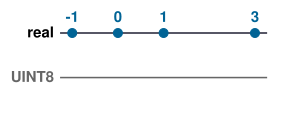
\includegraphics[width=0.92\textwidth,height=2.3cm,keepaspectratio]{numline_step1}}%
      \only<4-|handout:1>{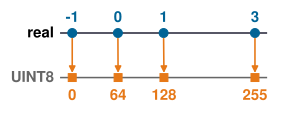
\includegraphics[width=0.92\textwidth,height=2.3cm,keepaspectratio]{numline_step2}}
    \end{column}
  \end{columns}
  \mlsyscredit{Model Compression, Napkin Math 10.1.}
  \note{[3 min] [CORE] Now the real size, by hand. ENGAGE: two minutes with a neighbor before any reveal; this is the toy grid with 8 bits instead of 3. Step 2: the scale is the range, \val{nm_range}, divided by \val{nm_steps} steps, about \val{nm_s}. Step 3: the zero-point is minus alpha over the scale: \val{nm_neg_alpha} divided by \val{nm_range}/\val{nm_steps} is \val{nm_z_exact}, rounded to \val{nm_z}. Step 4: each value divided by the scale, plus \val{nm_z}, rounded and clamped: $\val{nm_x0}$ maps to \val{nm_q0}, \val{nm_x1} to \val{nm_q1}, \val{nm_x2} to \val{nm_q2}, \val{nm_x3} to \val{nm_q3}. Why does it matter that real zero is exactly \val{nm_z}? Convolutions pad images with zeros, and ReLU produces many exact zeros; if zero did not land on an integer, every padded value would carry error. WARN: rounding \val{nm_z_exact} to \val{nm_z} nudges the whole grid by a quarter of a step, so $\val{nm_x0}$ reads back as $\val{nm_r0}$, not $\val{nm_x0}$; the zero-point is chosen to make zero exact at the cost of the endpoints. Students also forget the clamp, which stores anything outside $[\val{nm_alpha}, \val{nm_beta}]$ as 0 or \val{nm_steps}. LINK: the next slide runs the same tensor through PyTorch. FLEX: [CORE].}
\end{frame}

\begin{frame}[fragile]{PyTorch's observer picks the same scale, zero-point, and codes}
\vspace{-0.2cm}
\begin{semiverbatim}\footnotesize
u8 = torch.quint8
x = torch.tensor([[-1.0, 1.0], [0.0, 3.0]])
obs = MinMaxObserver(dtype=u8)
obs(x)
s, z = obs.calculate_qparams()
q = torch.quantize_per_tensor(x, s.item(), z.item(), u8)
\end{semiverbatim}
  \vspace{-0.25cm}
  \begin{columns}[T]
    \begin{column}{0.58\textwidth}
      {\footnotesize\textbf{Printed:} s, z; q.int\_repr(); q.dequantize()}
\vspace{-0.3cm}
\begin{semiverbatim}\footnotesize
0.01568627543747425 64
tensor([[  0, 128],
        [ 64, 255]], dtype=torch.uint8)
tensor([[-1.0039,  1.0039],
        [ 0.0000,  2.9961]])
\end{semiverbatim}
    \end{column}
    \begin{column}{0.40\textwidth}
      \small\textbf{By hand, last slide:}\\[0.05cm]
      $s = \val{nm_range}/\val{nm_steps} \approx \val{nm_s}$, \ $z = \val{nm_z}$\\[0.05cm]
      $X_q = \begin{pmatrix} \val{nm_q0} & \val{nm_q1} \\ \val{nm_q2} & \val{nm_q3} \end{pmatrix}$\\[0.05cm]
      $\val{nm_x0}$ reads back as $\val{nm_r0}$
    \end{column}
  \end{columns}
  \mlsyscredit{Run here: python -W ignore images/torch\_qparams.py (torch 2.13.0, CPU). Observer: torch/ao/quantization/observer.py (BSD-3).}
  \note{[1.5 min] Real tool output: this deck's images folder holds the script, and the text on the slide is what it printed (command: python -W ignore torch\_qparams.py, torch 2.13.0 on a CPU; the flag hides a deprecation notice for these quantized-tensor functions). A MinMaxObserver records the tensor's minimum and maximum and computes the scale and zero-point; its source, \_calculate\_qparams, does the focus slide's arithmetic: scale is the range over (quant\_max minus quant\_min), and zero\_point is quant\_min minus round(min over scale). quantize\_per\_tensor then stores the codes. Read the output against the hand calculation: scale \val{nm_s} (the float32 nearest \val{nm_range}/\val{nm_steps}), zero-point \val{nm_z}, codes \val{nm_q0}, \val{nm_q1}, \val{nm_q2}, and \val{nm_q3}, and $\val{nm_x0}$ reads back as $\val{nm_r0_torch}$, the quarter-step nudge from rounding \val{nm_z_exact} to \val{nm_z}. ENGAGE: if the tensor held only values from 0 to 3, which zero-point would the observer choose? Expected: 0, because real zero is then the bottom of the range. WARN: quint8 is unsigned, codes 0 to \val{nm_steps}; signed INT8 shifts every code by \val{int8_shift}. FLEX: [OPTIONAL]; cutting it loses the framework check of the worked example.}
\end{frame}

\begin{frame}{Inside the range, rounding misses by at most half a step}
  \begin{columns}[c]
    \begin{column}{0.52\textwidth}
      \centering\mlsyssteps[width=\textwidth,height=4.9cm,keepaspectratio]{rounderr_step}{2}
    \end{column}
    \begin{column}{0.46\textwidth}
      \centering\footnotesize
      Listing 2: symmetric INT8, $s = \val{l2_max} / \val{l2_int_max}$\\[0.1cm]
      \renewcommand{\arraystretch}{1.1}
      \begin{tabular}{@{}rrr@{}}
        \toprule
        \textbf{Weight} & \textbf{Code} & \textbf{Error} \\
        \midrule
        \val{l2_w0} & \val{l2_q0} & \val{l2_e0} \\
        $\val{l2_w1}$ & $\val{l2_q1}$ & \val{l2_e1} \\
        \val{l2_w2} & \val{l2_q2} & \val{l2_e2} \\
        $\val{l2_w3}$ & $\val{l2_q3}$ & \val{l2_e3} \\
        \bottomrule
      \end{tabular}\\[0.15cm]
      \small All below $s/2 = \val{l2_half}$.
    \end{column}
  \end{columns}
  \mlsyscredit{Model Compression, \S10.3.3 and listing 2; errors derived. Left: the 3-bit toy grid.}
  \note{[1.5 min] [CORE] Step 1: the error after a round trip (quantize, then read back) for every real value on the toy grid. Inside the range it is a sawtooth that never leaves the green band, because rounding to the nearest level misses by at most half a step, \val{toy_half} here. Step 2: outside the range the error is clipping, and it grows without limit, red. So the two failure modes differ in kind. Rounding error is bounded and small, clipping error is unbounded. Right: the chapter's listing 2, four real weights with the symmetric form (zero-point 0, scale set by the largest magnitude, \val{l2_max} / \val{l2_int_max} = \val{l2_s}). Codes \val{l2_q0}, $\val{l2_q1}$, \val{l2_q2}, $\val{l2_q3}$; every error is below half a step, \val{l2_half} (derived). ENGAGE: double the range to cover an outlier at \val{l2_outlier}. What happens to these errors? Expected: the step doubles, so the bound doubles, for every weight. That is the cost of covering outliers. FLEX: [CORE].}
\end{frame}

\begin{frame}{A zero-point buys back half the levels for one-sided data}
  \centering
  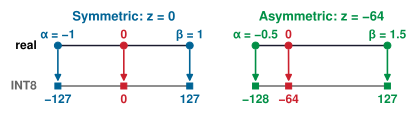
\includegraphics[width=0.86\textwidth,height=2.55cm,keepaspectratio]{calranges}\\[0.05cm]
  \uncover<2->{\small ReLU6 output, $[0, \val{relu_hi}]$: symmetric step $\val{relu_hi}/\val{relu_sym_div} = \val{relu_sym_s}$; asymmetric $\val{relu_hi}/\val{relu_asym_div} = \val{relu_asym_s}$.}\\[0.1cm]
  \uncover<3->{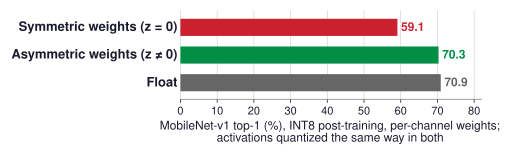
\includegraphics[width=0.80\textwidth,height=2.45cm,keepaspectratio]{zeropoint}}
  \mlsyscredit{Redrawn after Model Compression, \S10.3.3 (figure 22); $z = \val{zp_asym_z}$ and steps derived. Bars: Krishnamoorthi 2018, Table 3 (post-training INT8, per-channel weights, activations alike).}
  \note{[2 min] [OPTIONAL] Step 1, the book's figure redrawn. Left: symmetric, $[\val{zp_sym_lo}, \val{zp_sym_hi}]$ onto $\val{zp_sym_qmin}$ to \val{zp_sym_qmax}, zero-point 0. Right: asymmetric, $[\val{zp_asym_lo}, \val{zp_asym_hi}]$ onto $\val{zp_asym_qmin}$ to \val{zp_asym_qmax}; the step is \val{zp_asym_range}/\val{zp_asym_steps}, so real zero lands at code $\val{zp_asym_z}$ (derived). Step 2: after ReLU6 (MobileNet's activation, which clips outputs to 0 to \val{relu_hi}) every value is non-negative. A symmetric grid spends half its levels on negative values that never occur, so its step is \val{relu_hi}/\val{relu_sym_div} = \val{relu_sym_s}; an asymmetric grid spends all \val{relu_asym_div} steps on $[0, \val{relu_hi}]$, a step of \val{relu_asym_s}, half as large (derived). Step 3, measured: these bars compare weight grids; the activations are quantized the same way in both. With per-channel INT8 post-training weights, MobileNet-v1 reaches \val{mbv1_sym} percent on a symmetric grid and \val{mbv1_asym} on an asymmetric one, against \val{mbv1_float} in float. Even weights need not be centered; here a symmetric grid costs \val{mbv1_sym_cost} points. A nonzero zero-point has a cost. Every output needs a correction term, z times the sum of the weights. ENGAGE: why do many runtimes still default to symmetric weights and asymmetric activations? Expected: symmetric weights avoid the correction term, and quantization-aware training closes the symmetric gap (Krishnamoorthi 2018, \S3.2.3); activations after ReLU are one-sided. WARN: these bars show where symmetric weights fail; do not cite them for the default. FLEX: [OPTIONAL].}
\end{frame}

\begin{frame}{Integer layers add in 32 bits and rescale once per output}
  \centering
  \begin{tikzpicture}[node distance=0.45cm]
    \node[blk=BlueLine] (q) {Quantize\\$w$, $x$ to INT8};
    \node[blk=OrangeLine, right=of q] (m) {INT8 $\times$ INT8\\products};
    \node[blk=RedLine, right=of m] (a) {INT32\\accumulate};
    \node[blk=GreenLine, right=of a] (r) {$\times M$, round\\back to INT8};
    \draw[arr] (q) -- (m); \draw[arr] (m) -- (a); \draw[arr] (a) -- (r);
  \end{tikzpicture}\\[0.25cm]
  \footnotesize
  \renewcommand{\arraystretch}{1.12}
  \begin{tabular}{@{}lcccc@{}}
    \toprule
    $w$, \ $s_w = \val{il_w_max}/\val{il_int_max}$ & \val{il_w0} & $\val{il_w1}$ & \val{il_w2} & \\
    $x$, \ $s_x = \val{il_x_max}/\val{il_int_max}$ & \val{il_x0} & \val{il_x1} & \val{il_x2} & \\
    \midrule
    \uncover<2->{$w_q$, \ $x_q$} & \uncover<2->{\val{il_wq0}, \val{il_xq0}} & \uncover<2->{$\val{il_wq1}$, \val{il_xq1}} & \uncover<2->{\val{il_wq2}, \val{il_xq2}} & \\
    \uncover<3->{INT32 products, sum} & \uncover<3->{\val{il_p0}} & \uncover<3->{$\val{il_p1}$} & \uncover<3->{\val{il_p2}} & \uncover<3->{\textbf{\val{il_sum}}} \\
    \bottomrule
  \end{tabular}\\[0.2cm]
  \uncover<4->{\small $\val{il_sum} \times s_w s_x = \val{il_readback}$ \ (exact: \val{il_exact}). \quad $M = s_w s_x / s_y = \val{il_m}$, \ $y_q = \val{il_y}$.}
  \mlsyscredit{Pipeline after Model Compression, \S10.3.3 (figure 24, requantization scale $M$). Worked numbers derived; output scale $s_y = 1/\val{il_sy_div}$.}
  \note{[3 min] [CORE] One output of one INT8 layer, by hand. Step 1: quantize both inputs, multiply in pairs, add in a 32-bit integer register, then multiply once by a combined scale $M$. Each tensor's scale is its largest magnitude over \val{il_int_max}. Step 2: the codes. \val{il_w0} / (\val{il_w_max}/\val{il_int_max}) = \val{il_w0_ratio}, so \val{il_wq0}; $\val{il_w1}$ gives $\val{il_wq1}$; \val{il_w2} gives \val{il_wq2}. For $x$: \val{il_x0_ratio} rounds to \val{il_xq0}, then \val{il_xq1} and \val{il_xq2}. Step 3: integer products \val{il_p0}, $\val{il_p1}$, and \val{il_p2}, summed in INT32: \val{il_sum}. ENGAGE: why not add in 8 bits? Expected: one product already needs 15 to 16 bits, and a layer adds thousands of them. A 32-bit register holds about \val{il_headroom} worst-case products of $\val{il_int_max} \times \val{il_int_max}$ (derived: $2^{\val{il_acc_exp}} / \val{il_int_max}^2$). Step 4: reading the sum back as a real number multiplies by both scales, \val{il_readback}, against the exact \val{il_exact}; each rounding added a little. For the next layer, multiply by $M = s_w s_x / s_y$ = \val{il_m} and round: \val{il_y}. WARN: the scales apply once per output, which is why integer layers are cheap. Land the segment: two numbers per range define the mapping; inside the range the error is at most half a step; integer layers add in 32 bits and rescale once.}
\end{frame}

% =============================================================================
% SECTION: THE RANGE
% =============================================================================
\mlsysnote{[0.5 min] [CORE] The mapping is fixed by the range. Which range should one scale cover, and how many scales should a tensor get?}
\mlsysdivider{Which range should one scale cover?}{Model Compression, \S10.3.3 (calibration, granularity)}
\section{Range}

\begin{frame}{Clipping the tail gives the bulk \val{clip_finer}$\times$ finer steps}
  \mlsysactivity{Estimate}{1.5 min}
  \centering
  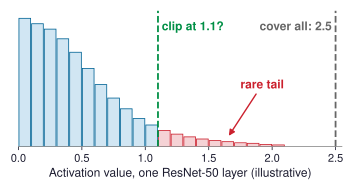
\includegraphics[width=0.86\textwidth,height=4.3cm,keepaspectratio]{calhist_step1}\\[0.05cm]
  \only<1|handout:0>{\normalsize UINT8 over $[0, \val{clip_full}]$, or clipped at \val{clip_cut}: step size of each? What happens above \val{clip_cut}?}%
  \only<2-|handout:1>{\small $\val{clip_full}/\val{clip_steps} = \val{clip_full_s}$ against $\val{clip_cut}/\val{clip_steps} = \val{clip_cut_s}$; values above \val{clip_cut} saturate at code \val{clip_steps}.}
  \mlsyscredit{Redrawn after Model Compression, \S10.3.3 (figure 21, after Wu et al. 2020; illustrative). Step sizes derived (images/calcs.py).}
  \note{[1.5 min] [CORE] Activations of one ResNet-50 layer, as the chapter draws them (illustrative): most values below about \val{clip_cut}, a sparse tail past 2. Calibration means running a small set of unlabeled inputs through the model and recording each tensor's values to choose its range. ENGAGE: one minute, compute both step sizes. Step 2: covering everything to \val{clip_full} gives a step of \val{clip_full_s}; clipping at \val{clip_cut} gives \val{clip_cut_s}, about \val{clip_finer} times finer for the bulk (derived). The price is that every value above \val{clip_cut} is stored as the top code, \val{clip_steps}. WARN: clipping is a bet that the tail does not matter; the chapter says task validation must check rare cases. LINK: the next slide shows the measured version of this histogram and three rules for choosing the clip. FLEX: [CORE].}
\end{frame}

\begin{frame}{Measured: no calibration rule is best for every network}
  \begin{columns}[c]
    \begin{column}{0.55\textwidth}
      \centering
      \begin{tikzpicture}
        \node[anchor=south west, inner sep=0] (img) at (0,0)
          {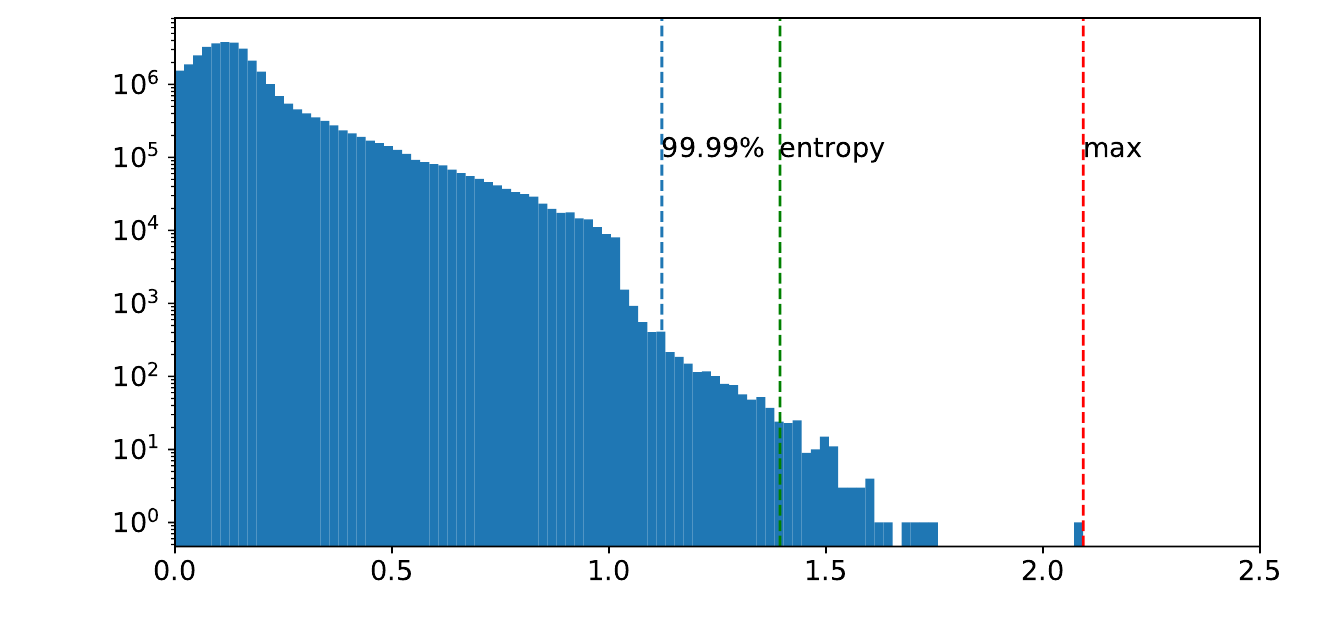
\includegraphics[width=\linewidth]{wu2020-fig2}};
        \begin{scope}[x={(img.south east)}, y={(img.north west)}]
          \fill[white] (0.498,0.715) rectangle (0.581,0.805);
          \fill[white] (0.590,0.715) rectangle (0.680,0.805);
          \node[font=\footnotesize\bfseries, text=BlueLine, fill=white, inner sep=1pt, anchor=west] at (0.497,0.88) {99.99\%};
          \node[font=\footnotesize\bfseries, text=GreenLine, fill=white, inner sep=1pt, anchor=west] at (0.592,0.76) {entropy};
          \node[font=\footnotesize\bfseries, text=RedLine, fill=white, inner sep=1pt, anchor=west] at (0.816,0.76) {max};
        \end{scope}
      \end{tikzpicture}\\[0.05cm]
      {\footnotesize ResNet-50 activations, log count, three ranges}
    \end{column}
    \begin{column}{0.43\textwidth}
      \centering\footnotesize
      \setlength{\tabcolsep}{3pt}
      \renewcommand{\arraystretch}{1.15}
      \begin{tabular}{@{}lrrrr@{}}
        \toprule
        \textbf{INT8} & \textbf{FP32} & \textbf{Max} & \textbf{Entr.} & \textbf{99.99\%} \\
        \midrule
        ResNet-50 & \val{wu_resnet50_fp32} & \val{wu_resnet50_max} & \textbf{\val{wu_resnet50_entropy}} & \val{wu_resnet50_pct_99_99} \\
        MobileNetV2 & \val{wu_mobilenet_fp32} & \val{wu_mobilenet_max} & \val{wu_mobilenet_entropy} & \textbf{\val{wu_mobilenet_pct_99_99}} \\
        Inception v4 & \val{wu_inception_fp32} & \textcolor{RedLine}{\val{wu_inception_max}} & \val{wu_inception_entropy} & \textbf{\val{wu_inception_pct_99_99}} \\
        EffNet-B0 & \val{wu_efficientnet_fp32} & \textcolor{RedLine}{\val{wu_efficientnet_max}} & \textbf{\val{wu_efficientnet_entropy}} & \val{wu_efficientnet_pct_99_99} \\
        BERT Large & \val{wu_bert_fp32} & \val{wu_bert_max} & \textcolor{RedLine}{\val{wu_bert_entropy}} & \val{wu_bert_pct_99_99} \\
        \bottomrule
      \end{tabular}\\[0.15cm]
      {\footnotesize Top-1 (BERT: F1); bold: best of the three}
    \end{column}
  \end{columns}
  \mlsyscredit{Wu, Judd, Zhang, Isaev, Micikevicius 2020 (arXiv 2004.09602): Figure 2 as published; Table 5 excerpt (weights per-channel max; activations calibrated as listed).}
  \note{[2 min] Measured, from the paper the chapter's histogram follows (Wu et al. 2020). Left, their Figure 2: the activations entering one ResNet-50 convolution, counts on a log scale, with the range each of three rules chooses. Max keeps the largest value seen and spends levels on a tail of a few single values. Percentile at 99.99 clips the top 0.01 percent of values; entropy picks the range whose rounded histogram stays closest to the original, by KL divergence. Both clip near the end of the bulk. Right, their Table 5: INT8 post-training accuracy, weights per channel, activations calibrated each way. ENGAGE: which rule would you make the default? Expected: none wins everywhere. Max collapses Inception v4 to \val{wu_inception_max} and EfficientNet-B0 to \val{wu_efficientnet_max}; entropy collapses BERT to \val{wu_bert_entropy}, where 99.99 percent nearly holds. The paper concludes that no single calibration is best for all networks, so calibrate per model and validate on the task. WARN: this ResNet-50 is v1.5 at \val{wu_resnet50_fp32}, a third checkpoint; compare within this table only. The paper's full table adds 99.9, 99.999, and 99.9999 percent; 99.999 is BERT's best, \val{wu_bert_best}. FLEX: [OPTIONAL]; cutting it loses the measured calibration comparison.}
\end{frame}

\begin{frame}{One scale per channel restores MobileNetV2 from \val{mbv2_tensor} to \val{mbv2_channel}\%}
  \centering
  \only<1-2|handout:0>{%
    \begin{tikzpicture}
      \node[anchor=south west, inner sep=0] (img) at (0,0)
        {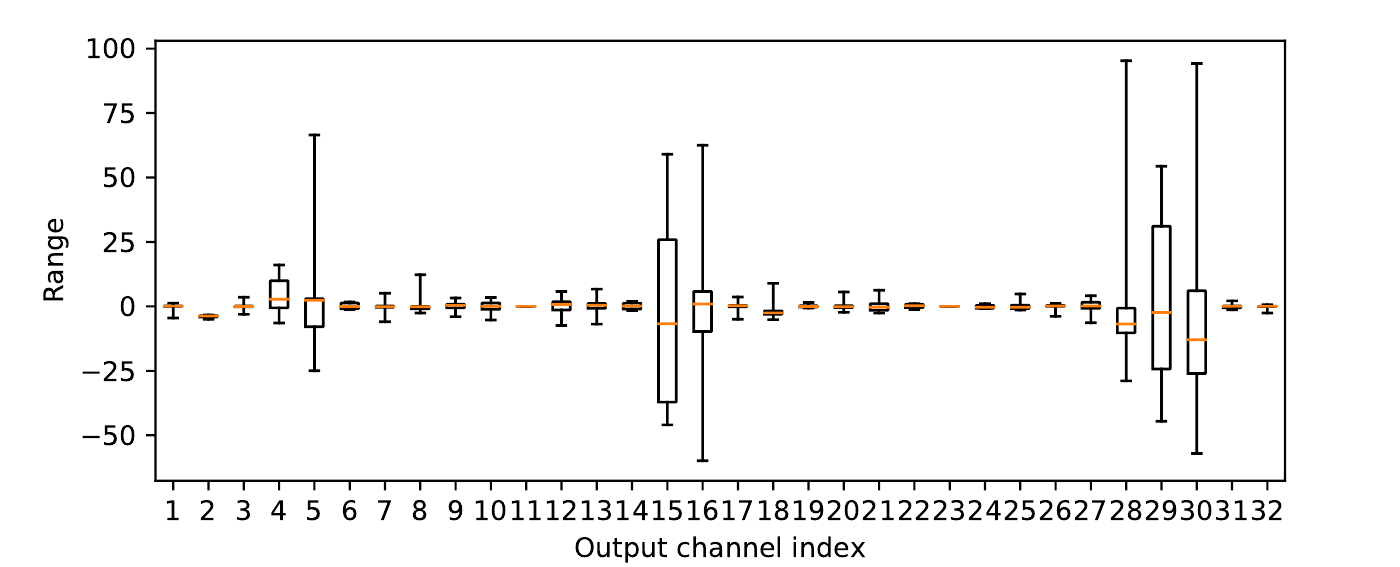
\includegraphics[width=11.4cm]{nagel2019-fig2}};
      \begin{scope}[x={(img.south east)}, y={(img.north west)}]
        \only<2>{%
          \draw[RedLine, line width=1.6pt, rounded corners=2pt] (0.465,0.17) rectangle (0.522,0.93);
          \draw[RedLine, line width=1.6pt, rounded corners=2pt] (0.791,0.17) rectangle (0.869,0.93);
          \draw[BlueLine, line width=1.6pt, rounded corners=2pt] (0.358,0.42) rectangle (0.392,0.50);
          \draw[BlueLine, line width=1.6pt, rounded corners=2pt] (0.661,0.42) rectangle (0.695,0.50);
          \node[font=\footnotesize\bfseries, text=RedLine, fill=white, inner sep=1.5pt, align=center]
            at (0.655,0.80) {wide channels\\set the scale};
          \node[font=\footnotesize\bfseries, text=BlueLine, fill=white, inner sep=1.5pt, anchor=north]
            at (0.53,0.33) {narrow: a few codes, or one};}
      \end{scope}
    \end{tikzpicture}}%
  \only<3-|handout:1>{\mlsyssteps[width=0.94\textwidth,height=4.6cm,keepaspectratio]{perchannel_step}{2}}\\[0.05cm]
  \only<1-2|handout:0>{\footnotesize Paper's example: channels in $[-\val{nagel_wide}, \val{nagel_wide}]$ and $(-\val{nagel_narrow}, \val{nagel_narrow})$; at 8 bits the second rounds to all zeros.}%
  \only<3-|handout:1>{\small No retraining needed; quantization-aware training adds \val{mbv2_qat_gain} points.}
  \mlsyscredit{Nagel, van Baalen, Blankevoort, Welling 2019 (arXiv 1906.04721), Figure 2 as published: per-output-channel weights of MobileNetV2's first depthwise layer. Bars: Krishnamoorthi 2018, Tables 3 and 4.}
  \note{[3.5 min] [CORE] The answer to the hook. Step 1, measured: Nagel et al.'s Figure 2, the weights of MobileNetV2's first depthwise layer (it filters each channel separately, Lecture 6), one box per output channel: minimum, quartiles, median, and maximum. Most of the \val{nagel_channels} channels sit close to zero; a few span tens of units. Step 2: one scale per tensor must cover the widest channels (red), so its step is large and a narrow channel's weights (blue) land on one or two codes. The paper's own example: a channel in $[-\val{nagel_wide}, \val{nagel_wide}]$ and one in $(-\val{nagel_narrow}, \val{nagel_narrow})$; with one 8-bit scale the step is about \val{nagel_step}, so every weight in the second becomes 0. Step 3: give each channel its own scale. Measured: MobileNetV2 goes from \val{mbv2_tensor} percent per-tensor to \val{mbv2_channel} per-channel with no retraining, and \val{mbv2_qat} with quantization-aware training (next segment), against \val{mbv2_float} in float. ResNet-50 stays at \val{r50_tensor} to \val{r50_float}. WARN: per-channel scales cost metadata and a rescale per channel; they are the default for weights, while activations usually keep one scale per tensor. Large language models go one step finer: one scale per group of weights, \val{awq_group} in AWQ (Lin et al. 2024) and \val{q4_block} in the GGUF block from the formats segment. The hook's answer: D. FLEX: [CORE].}
\end{frame}

\begin{frame}{Large language models grow outliers that break one scale per tensor}
  \centering
  \mlsyssteps[width=0.94\textwidth,height=4.7cm,keepaspectratio]{llmint8_step}{2}\\[0.05cm]
  \uncover<2->{\small LLM.int8() keeps the few outlier feature dimensions in 16 bits.}
  \mlsyscredit{Dettmers et al. 2022, Table 1 (C4 perplexity, dense transformers 125M to 13B; INT8 absmax) and \S1.}
  \note{[1.5 min] [OPTIONAL] Perplexity is the language model's average surprise at the next word; lower is better. Step 1: 32-bit float improves steadily with size. INT8 with one scale per tensor (absmax, set by the largest magnitude) stays close from \val{det_mid_b}B to \val{det_fourth_b}B, then breaks at \val{det_large_b}B: \val{det_absmax_large} against \val{det_fp32_large}. A few activation values far larger than the rest force one coarse per-tensor scale on everything else, the MobileNetV2 failure again, along a different axis. Step 2: LLM.int8() keeps those few feature dimensions in 16 bits and the rest in INT8, and matches float at 13B. WARN: the \val{det_small_m}M model also does badly under absmax (\val{det_absmax_small}); the paper's point is the trend at scale. LINK: the next slide shows where the outliers come from. FLEX: [OPTIONAL].}
\end{frame}

\begin{frame}{Outlier features appear abruptly near \val{out_b} billion parameters}
  \begin{columns}[c]
    \begin{column}{0.47\textwidth}
      \centering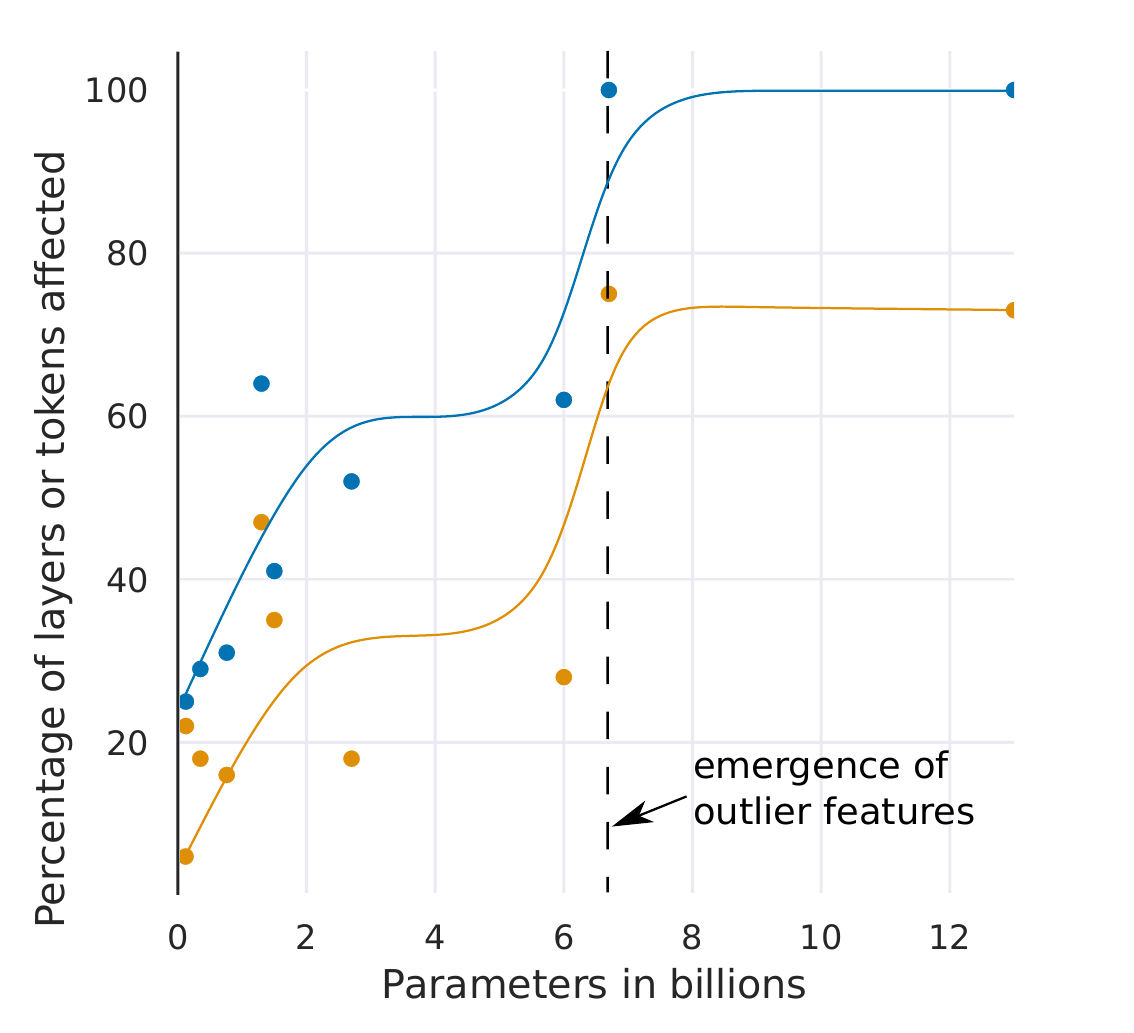
\includegraphics[width=\textwidth,height=5.9cm,keepaspectratio]{dettmers2022-fig3a}
    \end{column}
    \begin{column}{0.51\textwidth}
      \small
      \textcolor{BlueLine}{\textbf{Blue:}} share of layers with an outlier feature\\[0.1cm]
      \textcolor{OrangeLine}{\textbf{Orange:}} share of tokens affected\\[0.4cm]
      \uncover<2->{\normalsize From \val{out_b}B: every layer, about \val{out_tokens_pct}\% of tokens.\\[0.25cm]
      \small Values up to \val{out_mult}$\times$ the other features, in about \val{out_dims} hidden dimensions.}
    \end{column}
  \end{columns}
  \mlsyscredit{Dettmers et al. 2022 (LLM.int8(), arXiv 2208.07339), Figure 3(a) as published (legend from panel b); quantities from \S1.}
  \note{[1.5 min] [OPTIONAL] The cause behind the last slide's break at 13B, measured. An outlier feature is a hidden dimension whose activations reach a large magnitude (the paper's threshold is \val{out_threshold} or more) in many layers at once. Step 1: blue, the share of transformer layers where such features appear; orange, the share of token positions, across public language models from \val{det_small_m}M to \val{det_large_b}B parameters. Below about \val{out_floor_b} billion parameters they come and go. Step 2: near \val{out_b}B the paper reports a phase shift, in which every layer and about \val{out_tokens_pct} percent of positions are affected. The values reach up to \val{out_mult} times the rest, yet sit in only about \val{out_dims} hidden dimensions. ENGAGE: per-channel weight scales saved MobileNetV2. Why do they not save this model? Expected: these outliers are in the activations, so a weight scale cannot absorb them; LLM.int8() splits the matrix multiplication by feature and keeps those few columns in 16 bits. WARN: the curves are spline fits through a few models; read the jump and ignore the exact shape. FLEX: [OPTIONAL].}
\end{frame}

\begin{frame}{Diagnose: why does the INT8 model fail at night?}
  \mlsysactivity{Diagnose}{2.5 min}
  \begin{columns}[T]
    \begin{column}{0.48\textwidth}
      \begin{mlsyscard}{mlsysaccent}
        \textbf{Symptom (illustrative)}\\[0.1cm]
        \small Static INT8 ranges calibrated on 500 daytime images.\\[0.1cm]
        Night images: INT8 loses 6 points; FP32 loses 1.\\[0.1cm]
        Name two causes and two fixes.
      \end{mlsyscard}
    \end{column}
    \begin{column}{0.48\textwidth}
      \uncover<2->{\small
        \textbf{Cause:} ranges fixed on data that missed deployment; night values clip or use few levels.\\[0.15cm]
        \textbf{Fixes:} recalibrate with night images; compute ranges at run time; per-channel scales or quantization-aware training if still short.}
    \end{column}
  \end{columns}
  \mlsyscredit{Scenario illustrative. Model Compression, \S10.3.3 (static and dynamic ranges) and Checkpoint 10.2.}
  \note{[2.5 min] [CORE] ENGAGE: two minutes in pairs; ask for causes before fixes. The numbers are an invented scenario; say so. Step 2: the INT8 model has its activation ranges frozen from 500 daytime images (static quantization). Night images have darker inputs and different activation statistics. Some values fall outside the fixed range and clip, others sit in a small corner of it and get few levels. FP32 has no fixed range, so it degrades less. Fixes, in order of cost: recalibrate on a set that represents deployment, night included; dynamic quantization, which computes ranges per input at run time, costs a reduction pass over each activation tensor before the integer arithmetic; per-channel scales or quantization-aware training if post-training still misses. WARN: students answer ``use more bits''. That treats the symptom; the cause is the calibration data. Land the segment: the scale is set by the widest values it must cover, so clip rare outliers, give each channel its own scale, and treat the calibration set as part of the model.}
\end{frame}

% =============================================================================
% SECTION: THE LIMIT
% =============================================================================
\mlsysnote{[0.5 min] [CORE] Eight bits mostly work. How far down can we go, and what buys accuracy back?}
\mlsysdivider{How few bits before accuracy breaks, and what buys it back?}{Model Compression, \S10.3.3 (PTQ, QAT), \S10.3.4, \S10.3.5}
\section{Limit}

\begin{frame}{Eight bits stay on the accuracy plateau, and four bits fall off the cliff}
  \centering
  \mlsyssteps[width=0.95\textwidth,height=4.8cm,keepaspectratio]{cliff_step}{3}\\[0.05cm]
  \uncover<3->{\small With the same networks and 4-bit weights, retraining with rounding in the loop recovers most of it.}
  \mlsyscredit{Krishnamoorthi 2018, Tables 3 (8-bit weights and activations) and 5 (4-bit weights).}
  \note{[3 min] [CORE] Step 1: 8 bits, per-channel scales, no retraining: both networks within about \val{cliff_8bit_gap} points of float. Step 2: the same post-training method with 4-bit weights, \val{int4_levels} levels. With one scale per tensor both networks collapse to chance (\val{r50_w4_tensor} and \val{mbv2_w4_tensor}). Per-channel scales save ResNet-50 partly, \val{r50_w4_channel}, and MobileNetV2 not at all. This is the cliff the chapter describes, a plateau down to 8 bits, then a steep drop where \val{int4_levels} levels cannot represent the weights. ENGAGE: before step 3, what could recover it without more bits? Step 3: quantization-aware training (QAT), which fine-tunes the model with the rounding simulated in the forward pass so the weights move to where rounding hurts less: \val{r50_w4_qat} and \val{mbv2_w4_qat}. ResNet-50 is back within \val{r50_w4_qat_gap} points; MobileNetV2 is still \val{mbv2_w4_qat_gap} points short. WARN: the cliff's location is per model, per method; never assume it from another network. FLEX: binary and ternary networks (1 or 2 bits, multiply replaced by bit logic) are reading, \S10.3.4.}
\end{frame}

\begin{frame}{QAT rounds in the forward pass, passes gradients straight back}
  \centering
  \begin{tikzpicture}[node distance=0.5cm]
    \node[blk=BlueLine, minimum width=2.9cm] (p) {Pretrained\\model};
    \node[blk=OrangeLine, minimum width=2.9cm, right=of p] (f) {Insert fake\\quantization};
    \node[blk=RedLine, minimum width=2.9cm, right=of f] (t) {Fine-tune on\\training data};
    \node[blk=GreenLine, minimum width=2.9cm, right=of t] (q) {Quantized\\model};
    \draw[arr] (p) -- (f); \draw[arr] (f) -- (t); \draw[arr] (t) -- (q);
  \end{tikzpicture}\\[0.45cm]
  \begin{minipage}{0.92\textwidth}
    \small
    \textbf{Forward:} \ $\hat{x} = \operatorname{round}(x / s)\cdot s$\\[0.05cm]
    {\footnotesize The loss sees the rounding error deployment will see.}\\[0.25cm]
    \uncover<2->{\textbf{Backward:} \ $\dfrac{\partial \hat{x}}{\partial x} = 1$ inside $[\alpha, \beta]$, \ 0 outside\\[0.05cm]
    {\footnotesize Straight-through estimator: rounding's true gradient is 0 almost everywhere.}\\[0.3cm]}
    \centering\uncover<3->{\normalsize Try post-training first; pay for QAT only when it misses.}
  \end{minipage}
  \mlsyscredit{Pipeline after Model Compression, \S10.3.3 (figure 25 and training mathematics); straight-through estimator: Bengio et al. 2013.}
  \note{[1.5 min] [OPTIONAL] Top, the book's pipeline: a pretrained model, fake quantization inserted, then fine-tuning on the training data. Step 1: in the forward pass every weight and activation is quantized and read back (fake quantization), so the loss includes the rounding error. Step 2: the problem is the backward pass. Rounding is a staircase, so its derivative is 0 almost everywhere and gradients would vanish. The straight-through estimator treats rounding as the identity inside the clipping range and blocks the gradient outside it. The full-precision weights keep accumulating small updates until they cross a rounding threshold. Step 3: QAT needs the training data and a training run; post-training quantization needs only a small unlabeled calibration set and no training run. ENGAGE: a team has the checkpoint but not the training set. Which method? Expected: post-training only. WARN: the estimator is biased; QAT descends an approximation of the quantized loss.}
\end{frame}

\begin{frame}{GPTQ corrects rounding error as it goes}
  \centering
  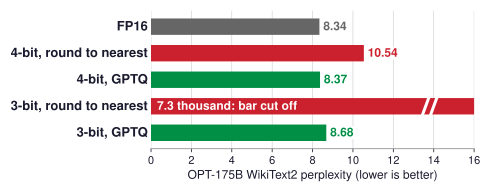
\includegraphics[width=0.90\textwidth,height=4.8cm,keepaspectratio]{gptq}\\[0.05cm]
  {\small GPTQ rounds each weight while correcting the error it leaves on the next ones.}
  \mlsyscredit{Frantar et al. 2023 (GPTQ), Table 5 (OPT-175B, WikiText2, weights only).}
  \note{[2 min] [OPTIONAL] Large language models cannot afford quantization-aware training at their size, so their low-bit methods are post-training and smarter about rounding. OPT-175B, weights only. Rounding each weight to the nearest 4-bit level raises perplexity from \val{gptq_fp16} to \val{gptq_rtn4}; GPTQ, which rounds the weights one at a time and adjusts the not-yet-rounded weights to cancel the error, gets \val{gptq_4}. At 3 bits round-to-nearest collapses to about \val{gptq_rtn3_k} thousand, while GPTQ holds \val{gptq_3}. ENGAGE: why can adjusting the remaining weights cancel error? Expected: the layer's output is a sum over weights times inputs, so an error in one term can be offset by small changes in the others. WARN: the \val{gptq_rtn3_k} thousand bar is cut off; perplexity that high means the model emits nonsense. FLEX: cutting it loses the GPTQ mechanism.}
\end{frame}

\begin{frame}{A weight matters by what it multiplies}
  \mlsysactivity{Predict}{2 min}
  \vspace{-0.1cm}
  \begin{mlsyscard}{BlueLine}
    \footnotesize\textbf{OPT-6.7B, INT3 weights, one scale per group of \val{awq_group} weights.} Keep \val{awq_kept_pct}\% of weights in FP16. Which 1\%: the largest weights, or those in channels with the largest activations?
  \end{mlsyscard}
  \centering\mlsyssteps[width=0.92\textwidth,height=3.75cm,keepaspectratio]{awq_step}{2}
  \mlsyscredit{Lin et al. 2024 (AWQ), Table 1 (INT3, groups of 128, WikiText perplexity).}
  \note{[2 min] [CORE] Step 1: ENGAGE, one minute. 3-bit OPT-6.7B, with one scale per group of \val{awq_group} weights, rounds to \val{awq_rtn} against \val{awq_fp16} in FP16. Keep \val{awq_kept_pct} percent of the weights in FP16. Most students choose the largest weights. Step 2: by weight size, \val{awq_by_weight}, close to plain rounding (\val{awq_rtn}); by activation size, \val{awq_by_act}, almost all the way back. A weight's effect on the output is weight times activation, so the weights that matter are those that multiply large activations. AWQ uses this. It scales those channels up before rounding instead of keeping them in FP16. Land the segment: eight bits sit on the plateau for most vision models; at four bits, rounding falls off a cliff unless training adapts the weights or the rounding protects the channels that matter. LINK: these are weight-only methods; the activations stay 16-bit, which matters for speed next.}
\end{frame}

% =============================================================================
% SECTION: THE SPEED
% =============================================================================
\mlsysnote{[0.5 min] [CORE] Fewer bits are on paper. When do they make the device faster?}
\mlsysdivider{When do fewer bits make the device faster?}{Model Compression, \S10.3.5, \S10.4.1, \S10.5.4}
\section{Speed}

\begin{frame}{Fewer bytes speed the slope; INT8 lifts the roof}
  \only<1-3|handout:0>{\mlsysactivity{Predict}{2 min}}
  \begin{columns}[c]
    \begin{column}{0.60\textwidth}
      \centering
      \only<1|handout:0>{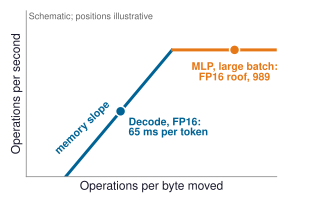
\includegraphics[width=\textwidth,height=5.3cm,keepaspectratio]{roofint_step1}}%
      \only<2|handout:0>{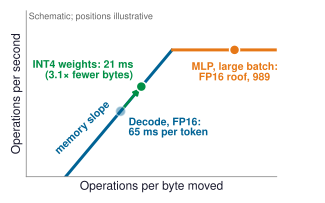
\includegraphics[width=\textwidth,height=5.3cm,keepaspectratio]{roofint_step2}}%
      \only<3-|handout:1>{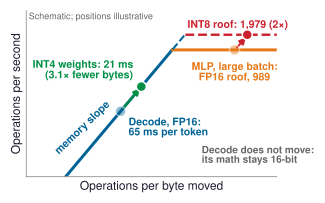
\includegraphics[width=\textwidth,height=5.3cm,keepaspectratio]{roofint_step3}}
    \end{column}
    \begin{column}{0.38\textwidth}
      \begin{mlsyscard}{BlueLine}
        \footnotesize\textbf{(a) GPT-2 XL decode, phone}\\ FP16 $\rightarrow$ INT4 weights, batch one\\
        \uncover<2->{\textbf{\val{dec_speedup}$\times$}: \val{dec_t16_gb} $\rightarrow$ \val{dec_t4_gb} GB per token}\\
        \uncover<4->{\textcolor{GreenLine}{Measured, OPT-175B 3-bit: \val{gptq_x}$\times$, \val{gptq_3bit_gpus_word} A100 against \val{gptq_fp16_gpus_word}}}
      \end{mlsyscard}
      \begin{mlsyscard}{OrangeLine}
        \footnotesize\textbf{(b) Large-batch MLP, H100}\\ FP16 $\rightarrow$ INT8\\
        \uncover<3->{\textbf{About \val{h100_int8_x}$\times$}: \val{h100_int8} against \val{h100_fp16} tera-ops/s}
      \end{mlsyscard}
    \end{column}
  \end{columns}
    \mlsyscredit{Model Compression, Napkin Math 10.2 and 10.4 (H100: NVIDIA 2022); roofline schematic, positions illustrative. Measured: Frantar et al. 2023, Table 6 (one A100 against five).}
  \note{[3.5 min] [CORE] Recall Lecture 2's roofline. Left of the bend, bytes moved set the time; right of it, arithmetic. Step 1: decoding GPT-2 XL at batch one on the phone reads every weight once per token, so it sits on the memory slope. Each token reads \val{dec_w16_gb} GB of FP16 weights plus a \val{dec_kv_gb} GB key-value (KV) cache, \val{dec_t16_gb} GB in all, \val{dec_t16_ms} ms. A large-batch MLP on the H100 reuses each weight and sits on the FP16 roof, \val{h100_fp16} tera-ops/s. ENGAGE: one minute, predict what INT4 weights do to the first point and INT8 to the second. Step 2: INT4 weights cut the bytes to \val{dec_t4_gb} GB per token, \val{dec_speedup} times fewer for the same operations, so the point slides up the slope: \val{dec_t4_ms} ms. Below \val{dec_byte_ratio} because the cache stayed FP16. Step 3: the H100's INT8 roof, \val{h100_int8}, twice FP16. The MLP point rises to it; decode does not move, since its math stays 16-bit. Step 4, measured: GPTQ's 3-bit OPT-175B runs at \val{gptq_3bit_ms} ms per token on \val{gptq_3bit_gpus_word} A100 against \val{gptq_fp16_ms} ms in FP16 on \val{gptq_fp16_gpus_word}, \val{gptq_x} times; say the change in GPU count aloud. WARN: on a chip without a faster integer path, case (b) gains nothing. LINK: the next slide measures both cases with one tool; Lecture 11 owns the roofline. FLEX: [CORE].}
\end{frame}

\begin{frame}[fragile]{Measured: 4-bit weights speed up generation and slow the prompt}
  {\footnotesize\textbf{llama-bench}, Llama 2 7B on an Apple M2 Ultra (\val{lb_ultra_bw} GB/s), build 8e672efe}
\begin{semiverbatim}\footnotesize
model                      size  test              t/s
llama 7B mostly F16   12.55 GiB  pp 512  1401.85 ± 1.75
llama 7B mostly F16   12.55 GiB  tg 128    41.02 ± 0.02
llama 7B mostly Q8_0   6.67 GiB  pp 512  1248.59 ± 0.73
llama 7B mostly Q8_0   6.67 GiB  tg 128    66.64 ± 0.02
llama 7B mostly Q4_0   3.56 GiB  pp 512  1238.48 ± 0.76
llama 7B mostly Q4_0   3.56 GiB  tg 128    94.27 ± 0.05
\end{semiverbatim}
  \vspace{-0.1cm}
  \begin{columns}[T]
    \begin{column}{0.49\textwidth}
      \uncover<2->{\begin{mlsyscard}{BlueLine}
        \footnotesize\textbf{Generate (tg 128): memory bound}\\
        Q4\_0: \textbf{\val{lb_tg4_x}$\times$} F16, from a file \val{lb_file_x}$\times$ smaller
      \end{mlsyscard}}
    \end{column}
    \begin{column}{0.49\textwidth}
      \uncover<2->{\begin{mlsyscard}{OrangeLine}
        \footnotesize\textbf{Prompt (pp 512): compute bound}\\
        Q4\_0: \textbf{\val{lb_pp4_x}$\times$} F16, slower
      \end{mlsyscard}}
    \end{column}
  \end{columns}
  \mlsyscredit{github.com/ggml-org/llama.cpp, discussion 4167 (M2 Ultra post, @ggerganov), llama-bench output; columns excerpted (every row: \val{llama_params_b} B weights, Metal, ngl 99). Ratios: images/calcs.py.}
  \note{[2.5 min] [CORE] Measured by a tool students can run on a laptop: llama-bench, from llama.cpp's public results thread. Every row is the same \val{llama_params_b}-billion-weight model on the GPU. tg 128 generates 128 tokens one at a time, batch one, like decoding on the phone; pp 512 processes a 512-token prompt in one pass. ENGAGE: from the roofline slide, which test should gain from Q4\_0, and by at most how much? Step 2: generation runs \val{lb_tg4_x} times faster with Q4\_0 (Q8\_0: \val{lb_tg8_x}) from a file \val{lb_file_x} times smaller, the memory-bound case, short of the byte ratio. The prompt runs \val{lb_pp4_x} times as fast because it is compute bound, so the 4-bit weights only add unpacking work. The thread's other chips agree, with generation \val{lb_other_tg_lo} to \val{lb_other_tg_hi} times on M1 Pro, M3 Max, and M4 Max, prompt \val{lb_other_pp_lo} to \val{lb_other_pp_hi} (derived). WARN: why short of \val{lb_file_x}? At F16 the M2 Ultra streams about \val{lb_stream16} GB/s of weights; at Q4\_0 about \val{lb_stream4} GB/s (derived: tokens per second times file size), so unpacking costs time on every byte. LINK: the next slide shows unpacking that costs more than it saves. FLEX: [CORE].}
\end{frame}

\begin{frame}{Unpacked in a separate pass, 4-bit weights move more than FP16}
  \centering
  \mlsyssteps[width=0.94\textwidth,height=4.6cm,keepaspectratio]{dequant_step}{2}\\[0.05cm]
  \uncover<2->{\small Unpack inside the matrix-multiply kernel, or lose the saving.}
  \mlsyscredit{Model Compression, Napkin Math 10.4, \S10.4.1, \S10.5.4. Separate-pass traffic derived; phone bus \val{phone_bw} GB/s.}
  \note{[2 min] Bytes per generated token for GPT-2 XL on the phone. Step 1: FP16, \val{dec_t16_gb} GB, \val{dec_t16_ms} ms; INT4 with the weights unpacked to 16 bits inside the matrix-multiply kernel (the compiled routine that runs the layer), in registers, as each tile arrives, so only the packed \val{dec_w4_gb} GB crosses the bus, \val{dec_t4_gb} GB in all, \val{dec_t4_ms} ms. ENGAGE: what if the runtime unpacks the weights in a separate kernel first? Step 2: it reads \val{dec_w4_gb} GB of packed weights, writes \val{dec_w16_gb} GB of FP16 weights back to memory, then the matrix multiply reads those \val{dec_w16_gb} GB again: \val{dq_sep_gb} GB with the cache, about \val{dq_sep_ms} ms, \val{dq_sep_x} times the FP16 time (derived). The same trap appears when an accelerator has INT8 matrix kernels but no INT8 LayerNorm: the runtime dequantizes, runs LayerNorm in floating point, and quantizes again (the chapter's runtime dequantization trap). WARN: a smaller file can run no faster; check the exported graph for separate dequantize kernels. LINK: Lecture 7's fusion rule, and Part 1's batch-norm folding. FLEX: [OPTIONAL]; cutting it loses the unpacking traffic.}
\end{frame}

\begin{frame}{INT8 opens the phone's DSP, and the DSP supplies most of the speed}
  \begin{columns}[c]
    \begin{column}{0.57\textwidth}
      \centering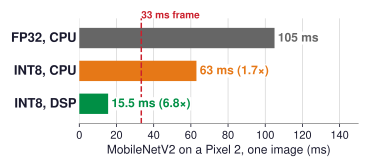
\includegraphics[width=\textwidth,height=3.8cm,keepaspectratio]{pixel2}\\[0.1cm]
      {\footnotesize Measured, MobileNetV2 classifier, Pixel 2}
    \end{column}
    \begin{column}{0.41\textwidth}
      \centering
      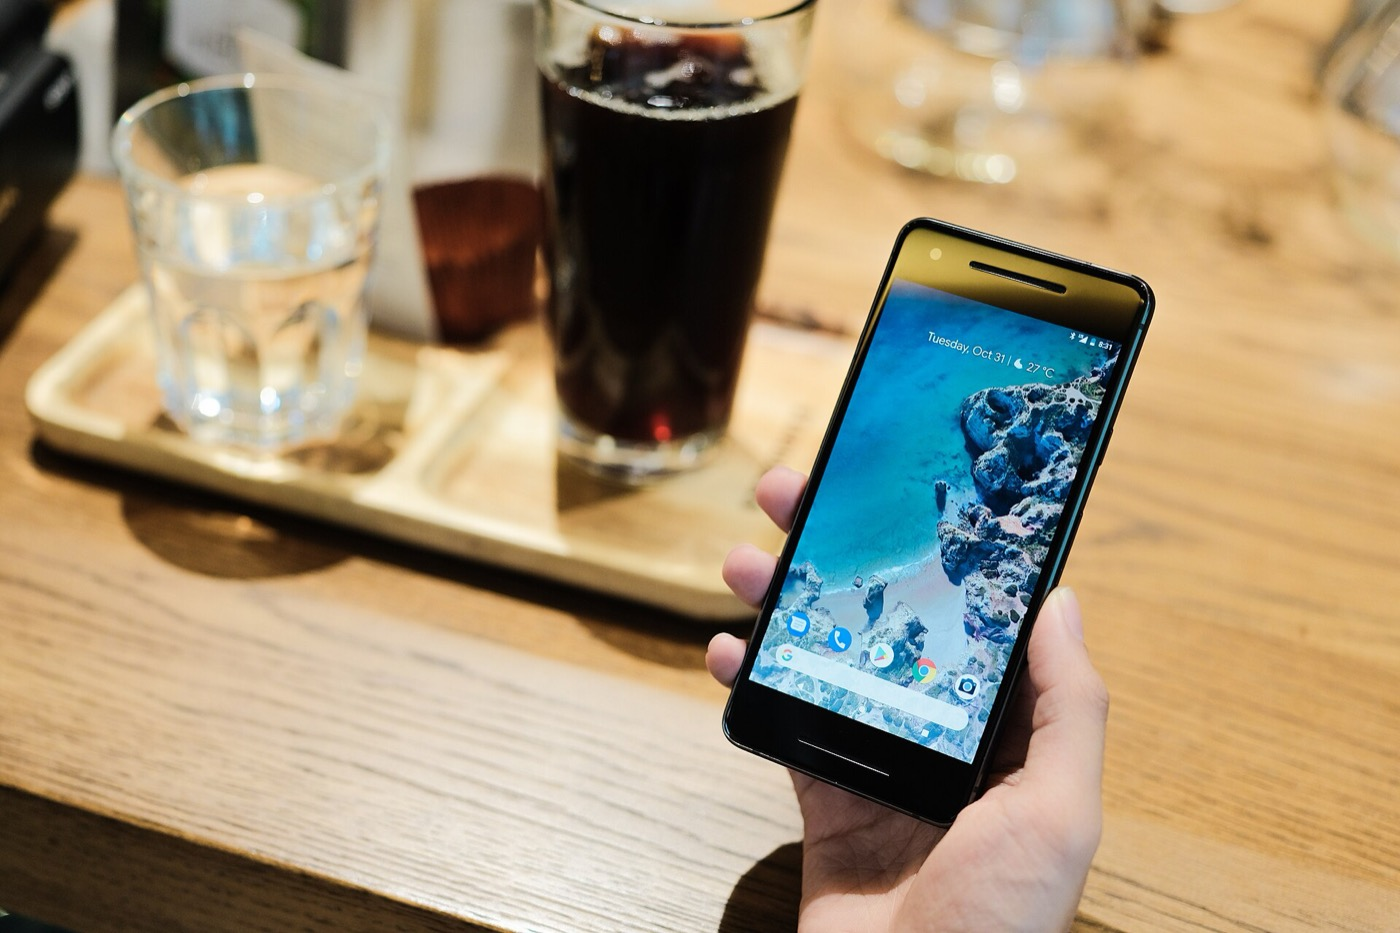
\includegraphics[width=\textwidth,height=4.0cm,keepaspectratio]{pixel2-phone}\\[0.1cm]
      {\footnotesize Pixel 2 (Snapdragon 835)}
    \end{column}
  \end{columns}
  \mlsyscredit{Krishnamoorthi 2018, Table 7 (one large CPU core; DSP via Android NN-API). Photo: Tinh t\'{\^e} Photo, CC0, Wikimedia Commons. Snapdragon 835: Wikipedia, ``Pixel 2''.}
  \note{[2.5 min] [CORE] Measured: MobileNetV2 on a Pixel 2, the phone on the right (photographed in 2017; its Snapdragon 835 chip holds the CPU cores and a Hexagon DSP). FP32 on one CPU core, \val{px_fp32} ms. INT8 on the same core, \val{px_cpu} ms, \val{px_cpu_x} times, because more 8-bit values fit in each vector register (Napkin Math 10.3: a \val{simd_bits}-bit register holds \val{simd_fp32} FP32 values or \val{simd_int8} INT8 values), and fewer bytes move. INT8 on the DSP (a digital signal processor beside the CPU, integer only), \val{px_dsp} ms, \val{px_dsp_x} times, under a \val{frame_ms} ms frame. Precision did not make the DSP faster; it made it usable. The chapter's illustrative blur pipeline makes the same argument. Pruning took the frame from \val{blur_cpu_ms} to \val{blur_pruned_ms} ms, and INT8 on the integer accelerator to about \val{blur_int8_ms} ms. ENGAGE: of the \val{px_dsp_x} times, how much is the bytes? Expected: at most the CPU's \val{px_cpu_x}; the rest is the processor. WARN: these numbers describe the classifier at 224 by 224; nobody measured the chapter's segmentation model this way. Land the segment: fewer bits speed a memory-bound layer by the bytes removed, if dequantization stays inside the kernel, and a compute-bound layer only through a faster integer path, often a different processor. FLEX: [CORE].}
\end{frame}

\begin{frame}{This INT8 profile is not yet evidence to ship}
  \mlsysactivity{Diagnose}{2.5 min}
  \centering\footnotesize
  \renewcommand{\arraystretch}{1.15}
  \begin{tabular}{@{}lll@{}}
    \toprule
    \textbf{ResNet-50, FP32 $\rightarrow$ INT8, H100} & \textbf{Result} & \uncover<3->{\textbf{What backs it}} \\
    \midrule
    Top-1 accuracy (limit \val{pf_top1_limit}\%) & \val{pf_fp32_top1} $\rightarrow$ \val{pf_int8_top1}\% & \uncover<3->{reported; passes} \\
    Confidence-calibration error (limit \val{pf_cal_limit}\%) & \val{pf_fp32_cal} $\rightarrow$ \textcolor{RedLine}{\val{pf_int8_cal}\%} & \uncover<3->{\textcolor{RedLine}{measured; \textbf{fails}}} \\
    Batch-one latency & \val{pf_latency_x}$\times$ & \uncover<3->{one engine profile, both precisions} \\
    Large-batch throughput & \val{pf_throughput_x}$\times$ & \uncover<3->{\textcolor{RedLine}{measured INT8 against modeled FP32}} \\
    Energy per image & \val{pf_energy_x}$\times$ & \uncover<3->{\textcolor{RedLine}{assumes \val{pf_tdp_w} W in both}} \\
    \uncover<3->{Tail latency, sustained power} & \uncover<3->{none} & \uncover<3->{\textcolor{RedLine}{not measured}} \\
    \bottomrule
  \end{tabular}\\[0.1cm]
  {\scriptsize Calibration error: how far predicted confidence is from observed accuracy.}\\[0.15cm]
  \uncover<2->{\normalsize Which claims are measured? Would you ship it?}
  \mlsyscredit{Model Compression, table 13 and \S10.6.2: the chapter's ResNet-50 checkpoint (\val{pf_fp32_top1}\%), not Krishnamoorthi's ResNet-v1-50 (\val{r50_float}\%) in the earlier bars.}
  \note{[2.5 min] [CORE] Step 1: the chapter's INT8 profile for ResNet-50 on the H100 (\val{pf_fp32_top1} percent, a different checkpoint from Krishnamoorthi's \val{r50_float}; do not compare). Step 2: ENGAGE, one minute in pairs: which numbers are evidence, and would you ship? Step 3: the backing. Accuracy passes the \val{pf_top1_limit} percent limit, and per-tensor INT8 suits ResNet-50, as segment 3 showed. Confidence-calibration error (predicted confidence against observed accuracy; not the range calibration of quantization) rises from \val{pf_fp32_cal} to \val{pf_int8_cal} percent against a \val{pf_cal_limit} percent limit, so it fails. Batch one gains only \val{pf_latency_x} times because launches, per-kernel floors, and the weight read dominate one image. The \val{pf_throughput_x} times throughput pairs an MLPerf (the industry benchmark suite, Lecture 12) INT8 measurement with a modeled FP32 rate from a different software stack, and the energy row assumes the board draws its full \val{pf_tdp_w} W in both precisions. Tail latency and sustained power are not in the profile. Expected verdict: no. Accuracy passes but calibration fails; recalibrate the confidences or quantize less aggressively, then remeasure both precisions on one stack (\S10.6.2). WARN: students treat the \val{pf_top1_drop}-point accuracy drop as the whole quality story. LINK: Lecture 11 (batch one), Lecture 12b (calibration error). FLEX: [CORE].}
\end{frame}

\begin{frame}[t]{True or false: four claims about quantization}
  \mlsysactivity{Vote}{2 min}
  \vspace{-0.45cm}
  \begin{columns}[T]
    \begin{column}{0.48\textwidth}
      \tfcard{INT8 post-training quantization costs at most a point.}{MobileNetV2, one scale per tensor: \val{mbv2_float} $\rightarrow$ \val{mbv2_tensor}\%.}\par\vspace{-0.3cm}
      \tfcard{INT4 weights make decoding \val{dec_byte_ratio}$\times$ faster.}{\val{dec_speedup}$\times$ on the phone; slower than FP16 if unpacked in a separate pass.}
    \end{column}
    \begin{column}{0.48\textwidth}
      \tfcard{Post-training quantization needs the labeled training set.}{A small unlabeled calibration set suffices.}\par\vspace{-0.3cm}
      \tfcard{Symmetric weight ranges are as good as asymmetric.}{MobileNet-v1, per-channel weights: \val{mbv1_sym} against \val{mbv1_asym}\%.}
    \end{column}
  \end{columns}
  \mlsyscredit{Krishnamoorthi 2018, Table 3; Model Compression, Napkin Math 10.4, \S10.3.3, \S10.7.}
  \note{[1.5 min] [OPTIONAL] Peer instruction: everyone votes true or false on all four, one minute with a neighbor, vote again. Step 2: all four are false. One: the hook, \val{mbv2_float} to \val{mbv2_tensor} percent; the chapter's fallacy ``aggressive quantization maintains performance'' sits here. Two: \val{dec_speedup} times, below \val{dec_byte_ratio} because the KV cache stays FP16, and a separate dequantize pass makes it slower than FP16. Three: post-training quantization calibrates ranges on a small unlabeled sample; quantization-aware training is the method that needs training data. Four: weight ranges need not be centered; with per-channel post-training weights, MobileNet-v1 reaches \val{mbv1_sym} percent on a symmetric grid against \val{mbv1_asym} on an asymmetric one, with the activations quantized the same way in both. WARN: if many voted true on one, return to the per-channel slide. FLEX: for a shorter lecture use claims one and two only.}
\end{frame}

% =============================================================================
% CLOSE
% =============================================================================
\begin{frame}{Back to MobileNetV2: \val{mbv2_tensor} to \val{mbv2_qat}\%, \val{px_fp32} to \val{px_dsp} ms}
  \begin{columns}[c]
    \begin{column}{0.50\textwidth}
      \centering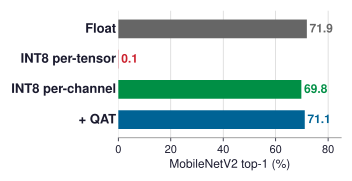
\includegraphics[width=\textwidth,height=4.0cm,keepaspectratio]{synth_acc}\\
      {\footnotesize One scale per channel, then QAT}
    \end{column}
    \begin{column}{0.48\textwidth}
      \centering
      \uncover<2->{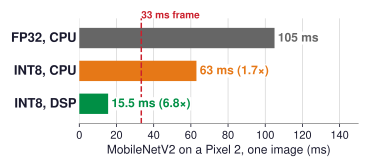
\includegraphics[width=\textwidth,height=2.8cm,keepaspectratio]{pixel2}\\
      {\footnotesize INT8 opens the DSP}\\[0.25cm]}
      \uncover<3->{\small Part 1's 7B model takes \val{p7b_int4_gb} GB of 4-bit codes and \val{p7b_q4_gb}~GB with block scales, so it fits in \val{phone_ram_gb} GB.}
    \end{column}
  \end{columns}
  \mlsyscredit{Krishnamoorthi 2018, Tables 3, 4, 7. 7B sizes derived (images/calcs.py): \val{p7b_b} billion $\times$ \val{int4_bytes} B; at Q4\_0's \val{q4_bpw} bits per weight, \val{p7b_q4_gb} GB.}
  \note{[1.5 min] [CORE] Return to the hook. Step 1: per-tensor INT8 took MobileNetV2 from \val{mbv2_float} to \val{mbv2_tensor} percent because one scale served channels with very different ranges. One scale per channel gave \val{mbv2_channel} percent with no retraining; quantization-aware training gave \val{mbv2_qat}. Step 2: the same INT8 model ran in \val{px_cpu} ms on the Pixel 2's CPU against \val{px_fp32} ms in FP32, and in \val{px_dsp} ms on the DSP, which cannot run FP32 at all. Precision enabled the speed, and the integer processor supplied most of it. Step 3: Part 1's \val{p7b_b}-billion-parameter model, \val{p7b_fp16_gb} GB in FP16, takes \val{p7b_int4_gb} GB of 4-bit codes, or \val{p7b_q4_gb} GB once the block scales from the GGUF slide are counted (derived), fits the phone's \val{phone_ram_gb} GB, and moves a quarter of the weight bytes per token when unpacking stays in the kernel. ENGAGE: which segment's idea fixed each problem? Expected: range granularity for MobileNetV2's accuracy, the integer processor for its speed, fused weight-only INT4 for the 7B model.}
\end{frame}

\begin{frame}{Takeaways}
  \vspace{-0.15cm}
  \thumbline{thumb_formats_step3}{An integer format keeps evenly spaced levels; a scale and a zero-point place them over a range.}\\[0.2cm]
  \thumbline{thumb_rounderr_step2}{Inside the range, error is at most half a step; clipping error is unbounded.}\\[0.2cm]
  \thumbline{thumb_perchannel_step2}{The widest values set the scale, so clip rare outliers and give channels their own scales.}\\[0.2cm]
  \thumbline{thumb_cliff_step3}{Eight bits sit on a plateau; below it, try post-training first, then QAT or activation-aware rounding.}\\[0.2cm]
  \thumbline{thumb_dequant_step2}{Fewer bits help a memory-bound layer by the bytes removed, if unpacking stays in the kernel.}
  \note{[1 min] [CORE] One line per idea, in segment order. Ask students to say which slide taught each. If short on time, read the first and last.}
\end{frame}

\begin{frame}{Open questions}
  \normalsize
  \begin{itemize}\setlength{\itemsep}{0.35cm}
    \item FP8 keeps an exponent and needs little calibration; INT8 needs careful ranges but smaller multipliers. If a phone accelerator could support only one, which should it be?
    \item Outlier features appear near \val{out_b}B parameters. Should models be trained to be easy to quantize, or should quantizers adapt to whatever training produces?
    \item A small set of calibration images now decides how a deployed model behaves on inputs it never saw. Who should own that data, and how should it be versioned?
  \end{itemize}
  \note{[1 min] [OPTIONAL] No single answer. Pick one for two minutes of discussion if time allows, or assign one as a short written response. The first previews Lecture 11 (datapaths) and Lecture 13 (runtime and precision selection); the third connects to Lecture 14 (operations).}
\end{frame}

\begin{frame}{Read and explore}
  \footnotesize
  \begin{itemize}\setlength{\itemsep}{0cm}
    \item \textbf{Read:} Model Compression, \S10.3, \S10.4.1, \S10.5.4, \S10.6.2 (mlsysbook.ai).
    \item Krishnamoorthi, ``Quantizing Deep Convolutional Networks for Efficient Inference: A Whitepaper,'' 2018.
    \item Jacob et al., ``Quantization and Training of Neural Networks for Integer-Arithmetic-Only Inference,'' CVPR 2018.
    \item Nagel et al., ``Data-Free Quantization Through Weight Equalization and Bias Correction,'' ICCV 2019.
    \item Nagel et al., ``A White Paper on Neural Network Quantization,'' 2021.
    \item Dettmers et al., ``LLM.int8(): 8-bit Matrix Multiplication for Transformers at Scale,'' NeurIPS 2022.
    \item Frantar et al., ``GPTQ: Accurate Post-Training Quantization for Generative Pre-trained Transformers,'' ICLR 2023.
    \item Lin et al., ``AWQ: Activation-aware Weight Quantization for On-Device LLM Compression,'' MLSys 2024.
  \end{itemize}
  \note{[0.5 min] [OPTIONAL] The chapter first: work Napkin Math 10.1 to 10.4 by hand and redo 10.4 for INT8 weights. Krishnamoorthi is the source of today's MobileNetV2 and Pixel 2 numbers; Jacob et al. is the scale-and-zero-point scheme mobile runtimes use; Nagel et al. 2019 is the source of the per-channel range finding, and Nagel et al. 2021 is a clear walk through the whole pipeline; Dettmers et al., Frantar et al., and Lin et al. are the three language-model papers. FLEX: add the TinyTorch quantization module if your course assigns it.}
\end{frame}

\begin{frame}[c]
  \begin{columns}[c]
    \begin{column}{0.34\textwidth}
      \centering\mlsysphoto[width=\textwidth,height=3.6cm,keepaspectratio]{nvidia-h100-pcie.jpg}
    \end{column}
    \begin{column}{0.62\textwidth}
      {\small\textcolor{lightgray}{NEXT LECTURE \textbar{} HARDWARE ACCELERATION, PART 1}}\\[0.5cm]
      {\LARGE\bfseries Why does moving data cost more than computing it?}
    \end{column}
  \end{columns}
  \mlsyscredit{Photo: Geekerwan (CC BY 3.0), Wikimedia Commons.}
  \note{[0.5 min] [CORE] The same INT8 change gave ResNet-50 \val{pf_latency_x} times at batch one and \val{pf_throughput_x} times at large batch on one chip, and decoding sped up by the bytes it stopped moving. Lecture 11 opens the accelerator to show why, and owns the roofline, the energy ladder, and the integer and sparse datapaths used today.}
\end{frame}

\end{document}
